\chapter{Appendix III}
\label{cha:AppendixIII}
%\addcontentsline{toc}{chapter}{\quad\,\,{Appendix II}}
\begin{singlespacing}

%	\section{Root mean square fluctuation (RMSF) of the backbone atoms per residue}
%	\label{sec:allrmsf}

	
%\newpage	
	\section{Formation and change in cavity volume in PKS ACPs over time}
	\label{sec:AppII:MDApoACP-mupA3a}

		\setlength\fboxsep{5pt}
		\setlength\fboxrule{1.5pt}
		\begin{figure}[htbp]
		\centering
		\fbox{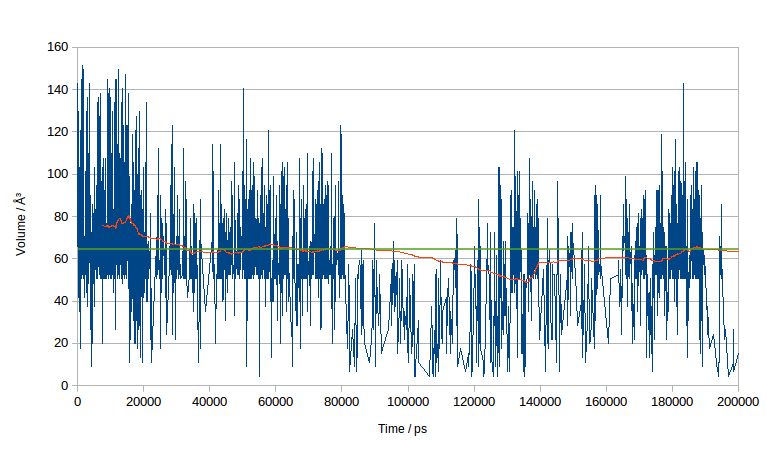
\includegraphics[width=0.9\textwidth, keepaspectratio=true]{graphics/CavityVolumeACPWild_nonzero.png}}
		\caption[Formation and change in cavity volume over time (200 ns) in the apo ACP-mupA3a WT.]{Formation and change in cavity volume over time (200 ns) in the apo ACP-mupA3a WT. The time frames which had a zero value for the volume were omitted from the plot. Red line represents the running average over 500 frames and green line represents the mean.}
		\label{fig:CavityVolumeACPWild_nonzero}
		\end{figure}

		\setlength\fboxsep{5pt}
		\setlength\fboxrule{1.5pt}
		\begin{figure}[htbp]
		\centering
		\fbox{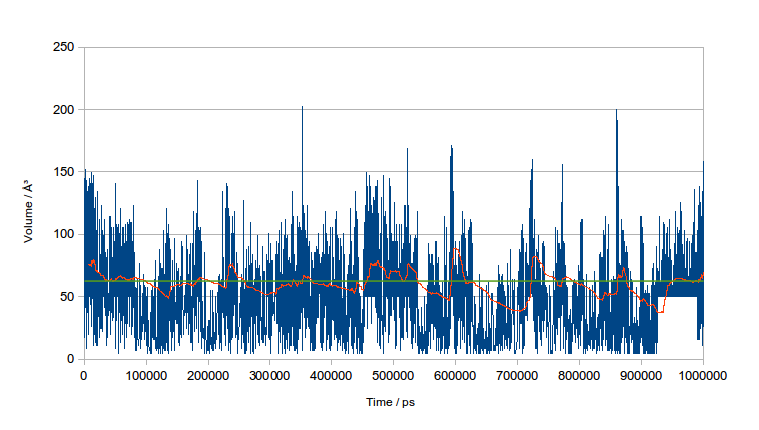
\includegraphics[width=0.9\textwidth, keepaspectratio=true]{graphics/CavityVolumeACPWild1000_nonzero.png}}
		\caption[Formation and change in cavity volume over time (1 $ \mu $s) in the apo ACP-mupA3a WT.]{Formation and change in cavity volume over time (1 $ \mu $s) in the apo ACP-mupA3a WT. The time frames which had a zero value for the volume were omitted from the plot. Red line represents the running average over 500 frames and green line represents the mean.}
		\label{fig:CavityVolumeACPWild1000_nonzero}
		\end{figure}		

		\setlength\fboxsep{5pt}
		\setlength\fboxrule{1.5pt}
		\begin{figure}[htbp]
		\centering
		\fbox{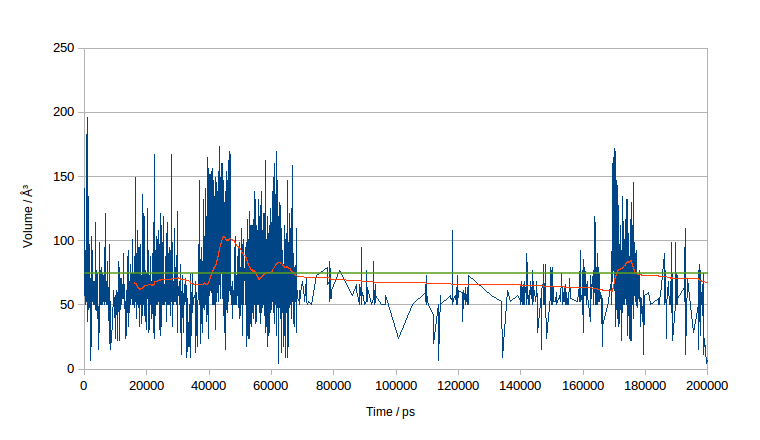
\includegraphics[width=0.9\textwidth, keepaspectratio=true]{graphics/CalvityVolumeACPMutant_nonzero.png}}
		\caption[Formation and change in cavity volume over time in the apo ACP-mupA3a W44L.]{Formation and change in cavity volume over time in the apo ACP-mupA3a W44L. The time frames which had a zero value for the volume were omitted from the plot. Red line represents the running average over 500 frames and green line represents the mean.}
		\label{fig:CalvityVolumeACPMutant_nonzero}
		\end{figure}		

		\setlength\fboxsep{5pt}
		\setlength\fboxrule{1.5pt}
		\begin{figure}[htbp]
		\centering
		\fbox{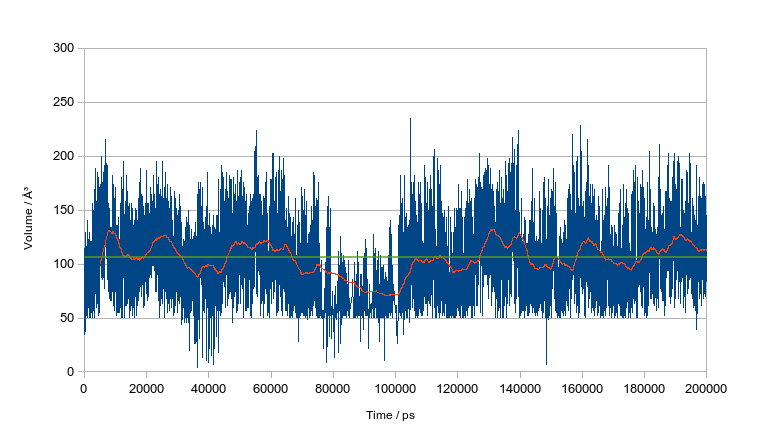
\includegraphics[width=0.9\textwidth, keepaspectratio=true]{graphics/CavityVolumeACPPPTWild_nonzero.png}}
		\caption[Formation and change in cavity volume over time in the holo ACP-mupA3a WT.]{Formation and change in cavity volume over time in the holo ACP-mupA3a WT. The time frames which had a zero value for the volume were omitted from the plot. Red line represents the running average over 500 frames and green line represents the mean.}
		\label{fig:CavityVolumeACPPPTWild_nonzero}
		\end{figure}

		\setlength\fboxsep{5pt}
		\setlength\fboxrule{1.5pt}
		\begin{figure}[htbp]
		\centering
		\fbox{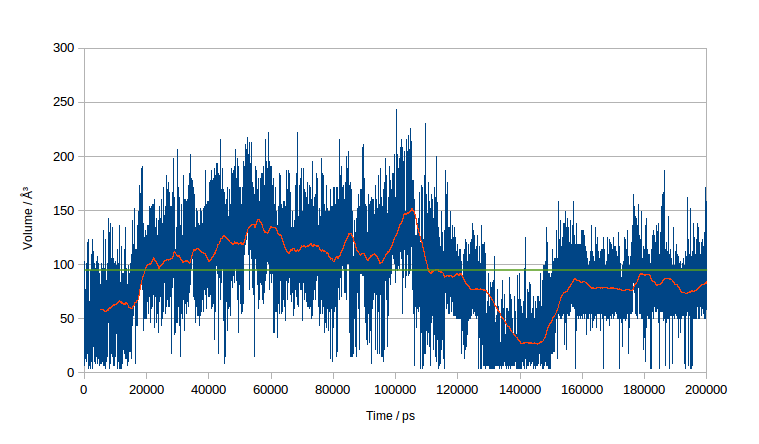
\includegraphics[width=0.9\textwidth, keepaspectratio=true]{graphics/CavityVolumeACPPPTMutant_nonzero.png}}
		\caption[Formation and change in cavity volume over time in the holo ACP-mupA3a W44L.]{Formation and change in cavity volume over time in the holo ACP-mupA3a W44L. The time frames which had a zero value for the volume were omitted from the plot. Red line represents the running average over 500 frames and green line represents the mean.}
		\label{fig:CavityVolumeACPPPMutant_nonzero}
		\end{figure}	

		\setlength\fboxsep{5pt}
		\setlength\fboxrule{1.5pt}
		\begin{figure}[htbp]
		\centering
		\fbox{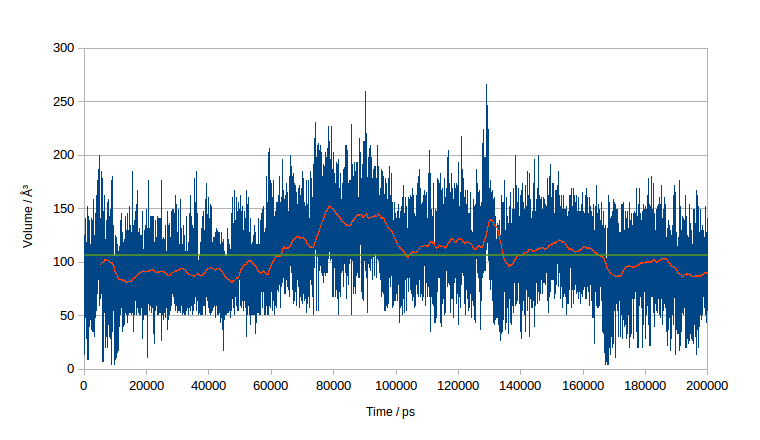
\includegraphics[width=0.9\textwidth, keepaspectratio=true]{graphics/CavityVolumeACPSPMWild200_nonzero.png}}
		\caption[Formation and change in cavity volume over time (200ns) in the acyl ACP-mupA3a WT.]{Formation and change in cavity volume over time (200ns) in the acyl ACP-mupA3a WT. The time frames which had a zero value for the volume were omitted from the plot. Red line represents the running average over 500 frames and green line represents the mean.}
		\label{fig:CavityVolumeACPSPMWild200_nonzero}
		\end{figure}

		\setlength\fboxsep{5pt}
		\setlength\fboxrule{1.5pt}
		\begin{figure}[htbp]
		\centering
		\fbox{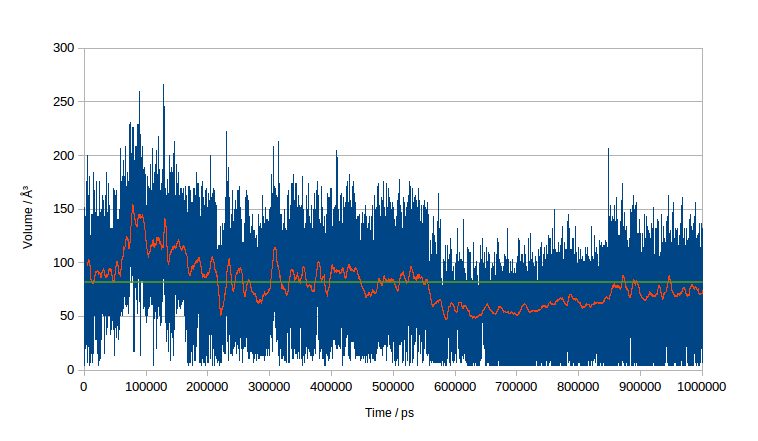
\includegraphics[width=0.9\textwidth, keepaspectratio=true]{graphics/CavityVolumeACPSPMWild1000_nonzero.png}}
		\caption[Formation and change in cavity volume over time (1 $ \mu $s) in the acyl ACP-mupA3a WT.]{Formation and change in cavity volume over time (1 $ \mu $s) in the acyl ACP-mupA3a WT. The time frames which had a zero value for the volume were omitted from the plot. Red line represents the running average over 500 frames and green line represents the mean.}
		\label{fig:CavityVolumeACPSPMWild1000_nonzero}
		\end{figure}
				

		\setlength\fboxsep{5pt}
		\setlength\fboxrule{1.5pt}
		\begin{figure}[htbp]
		\centering
		\fbox{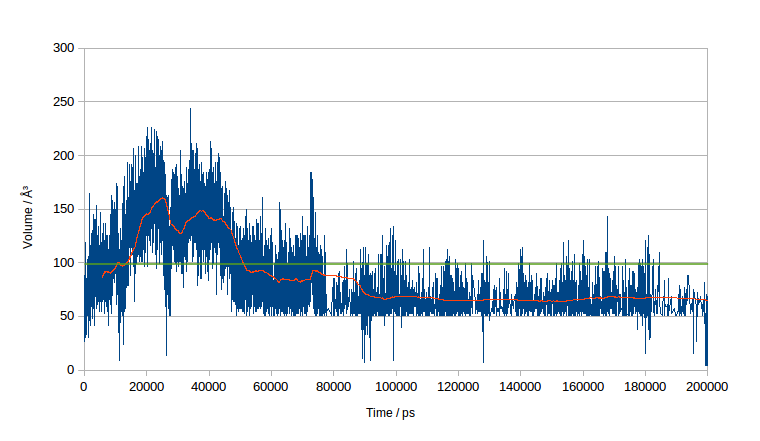
\includegraphics[width=0.9\textwidth, keepaspectratio=true]{graphics/CavityVolumeACPSPMMutant_nonzero.png}}
		\caption[Formation and change in cavity volume over time in the acyl ACP-mupA3a W44L.]{Formation and change in cavity volume over time in the acyl ACP-mupA3a W44L. The time frames which had a zero value for the volume were omitted from the plot. Red line represents the running average over 500 frames and green line represents the mean.}
		\label{fig:CavityVolumeACPSPMMutant_nonzero}
		\end{figure}		

		\setlength\fboxsep{5pt}
		\setlength\fboxrule{1.5pt}
		\begin{figure}[htbp]
		\centering
		\fbox{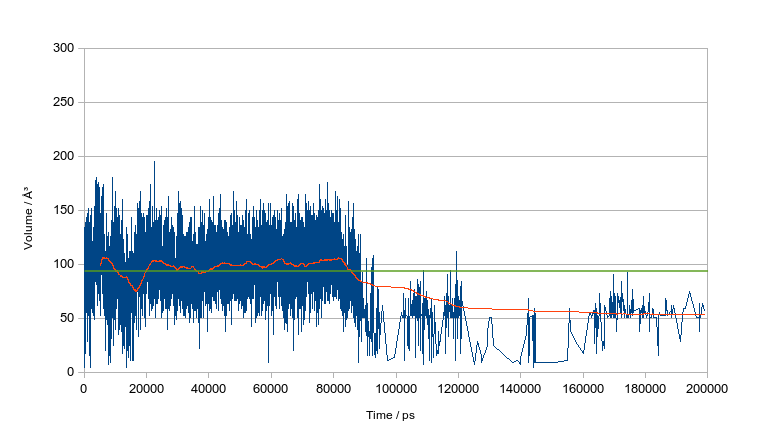
\includegraphics[width=0.9\textwidth, keepaspectratio=true]{graphics/CavityVolumeACPSPD_nonzero.png}}
		\caption[Formation and change in cavity volume over time in the acyl 14C ACP-mupA3a.]{Formation and change in cavity volume over time in the acyl 14C ACP-mupA3a. The time frames which had a zero value for the volume were omitted from the plot. Red line represents the running average over 500 frames and green line represents the mean.}
		\label{fig:CavityVolumeACPSPD_nonzero}
		\end{figure}
		
		\setlength\fboxsep{5pt}
		\setlength\fboxrule{1.5pt}
		\begin{figure}[htbp]
		\centering
		\fbox{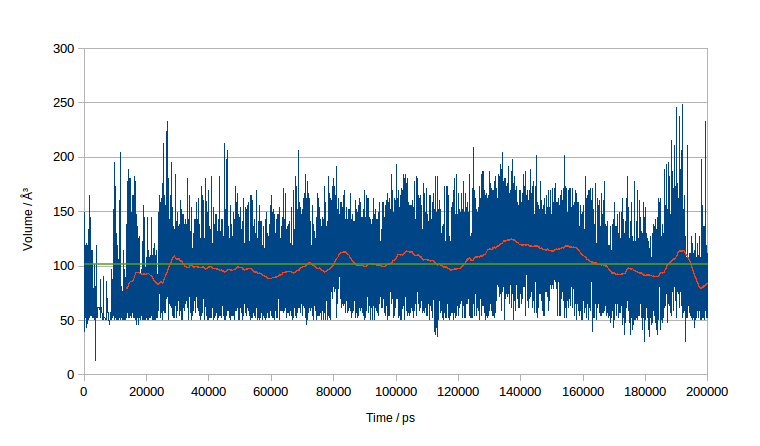
\includegraphics[width=0.9\textwidth, keepaspectratio=true]{graphics/CavityVolumeACP2_nonzero.png}}
		\caption[Formation and change in cavity volume over time in the acyl ACP-mupA2a.]{Formation and change in cavity volume over time in the acyl ACP-mupA2a. The time frames which had a zero value for the volume were omitted from the plot. Red line represents the running average over 500 frames and green line represents the mean.}
		\label{fig:CavityVolumeACP2_nonzero}
		\end{figure}		
		
		\setlength\fboxsep{5pt}
		\setlength\fboxrule{1.5pt}
		\begin{figure}[htbp]
		\centering
		\fbox{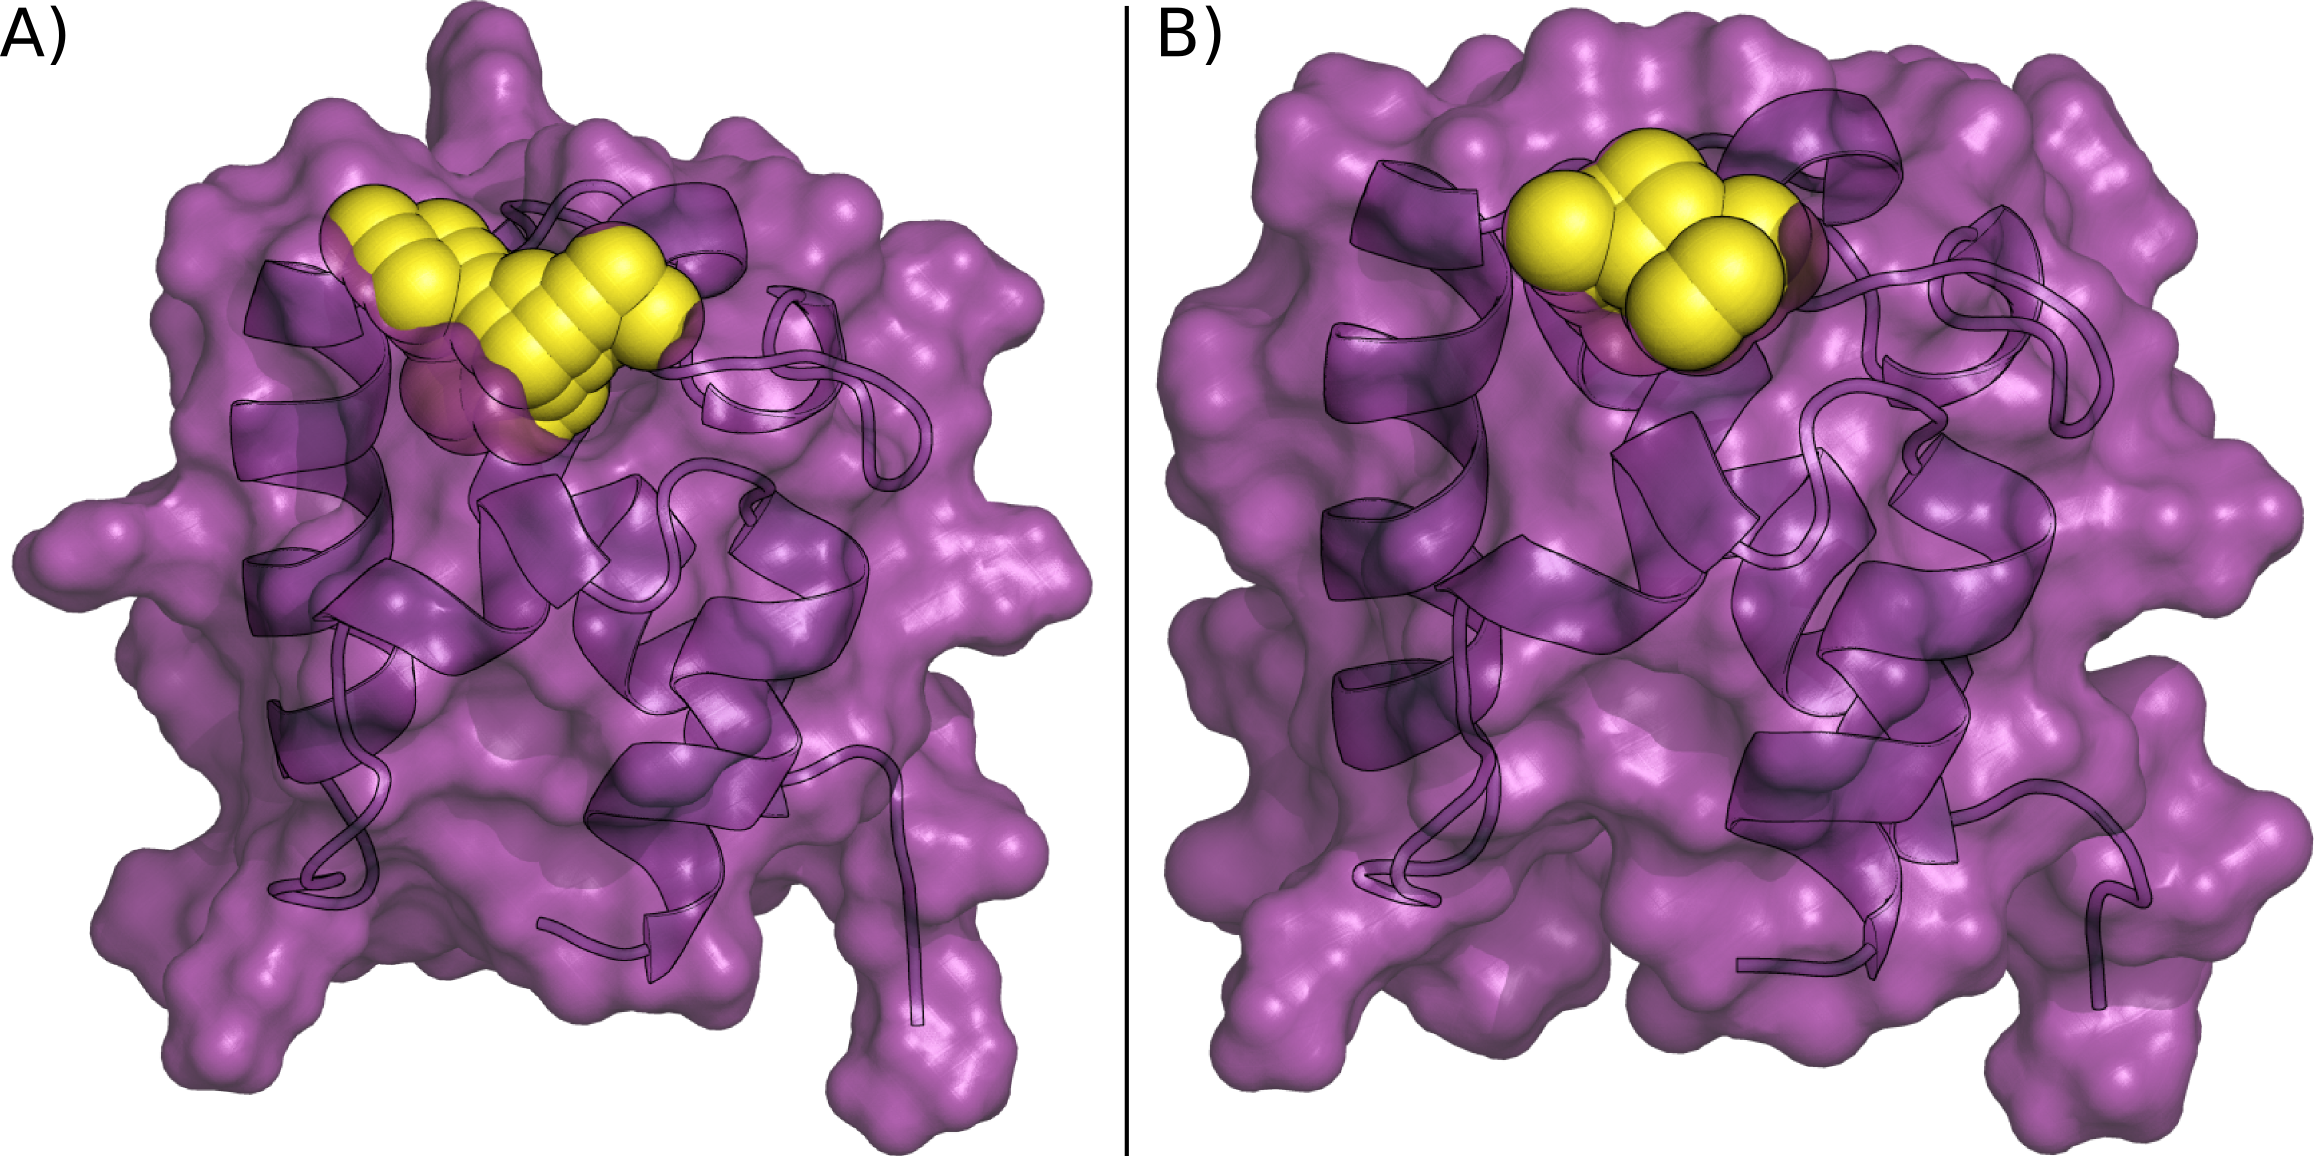
\includegraphics[width=0.9\textwidth, keepaspectratio=true]{graphics/acp_wild.png}}
		\caption[Space filled diagram of the largest and the modal cavity volume in the apo ACP-mupA3a WT.]{Space filled diagram of the largest (A) and the modal (B) cavity volume in the apo ACP-mupA3a WT.}
		\label{fig:acp_wild}
		\end{figure}

		\setlength\fboxsep{5pt}
		\setlength\fboxrule{1.5pt}
		\begin{figure}[htbp]
		\centering
		\fbox{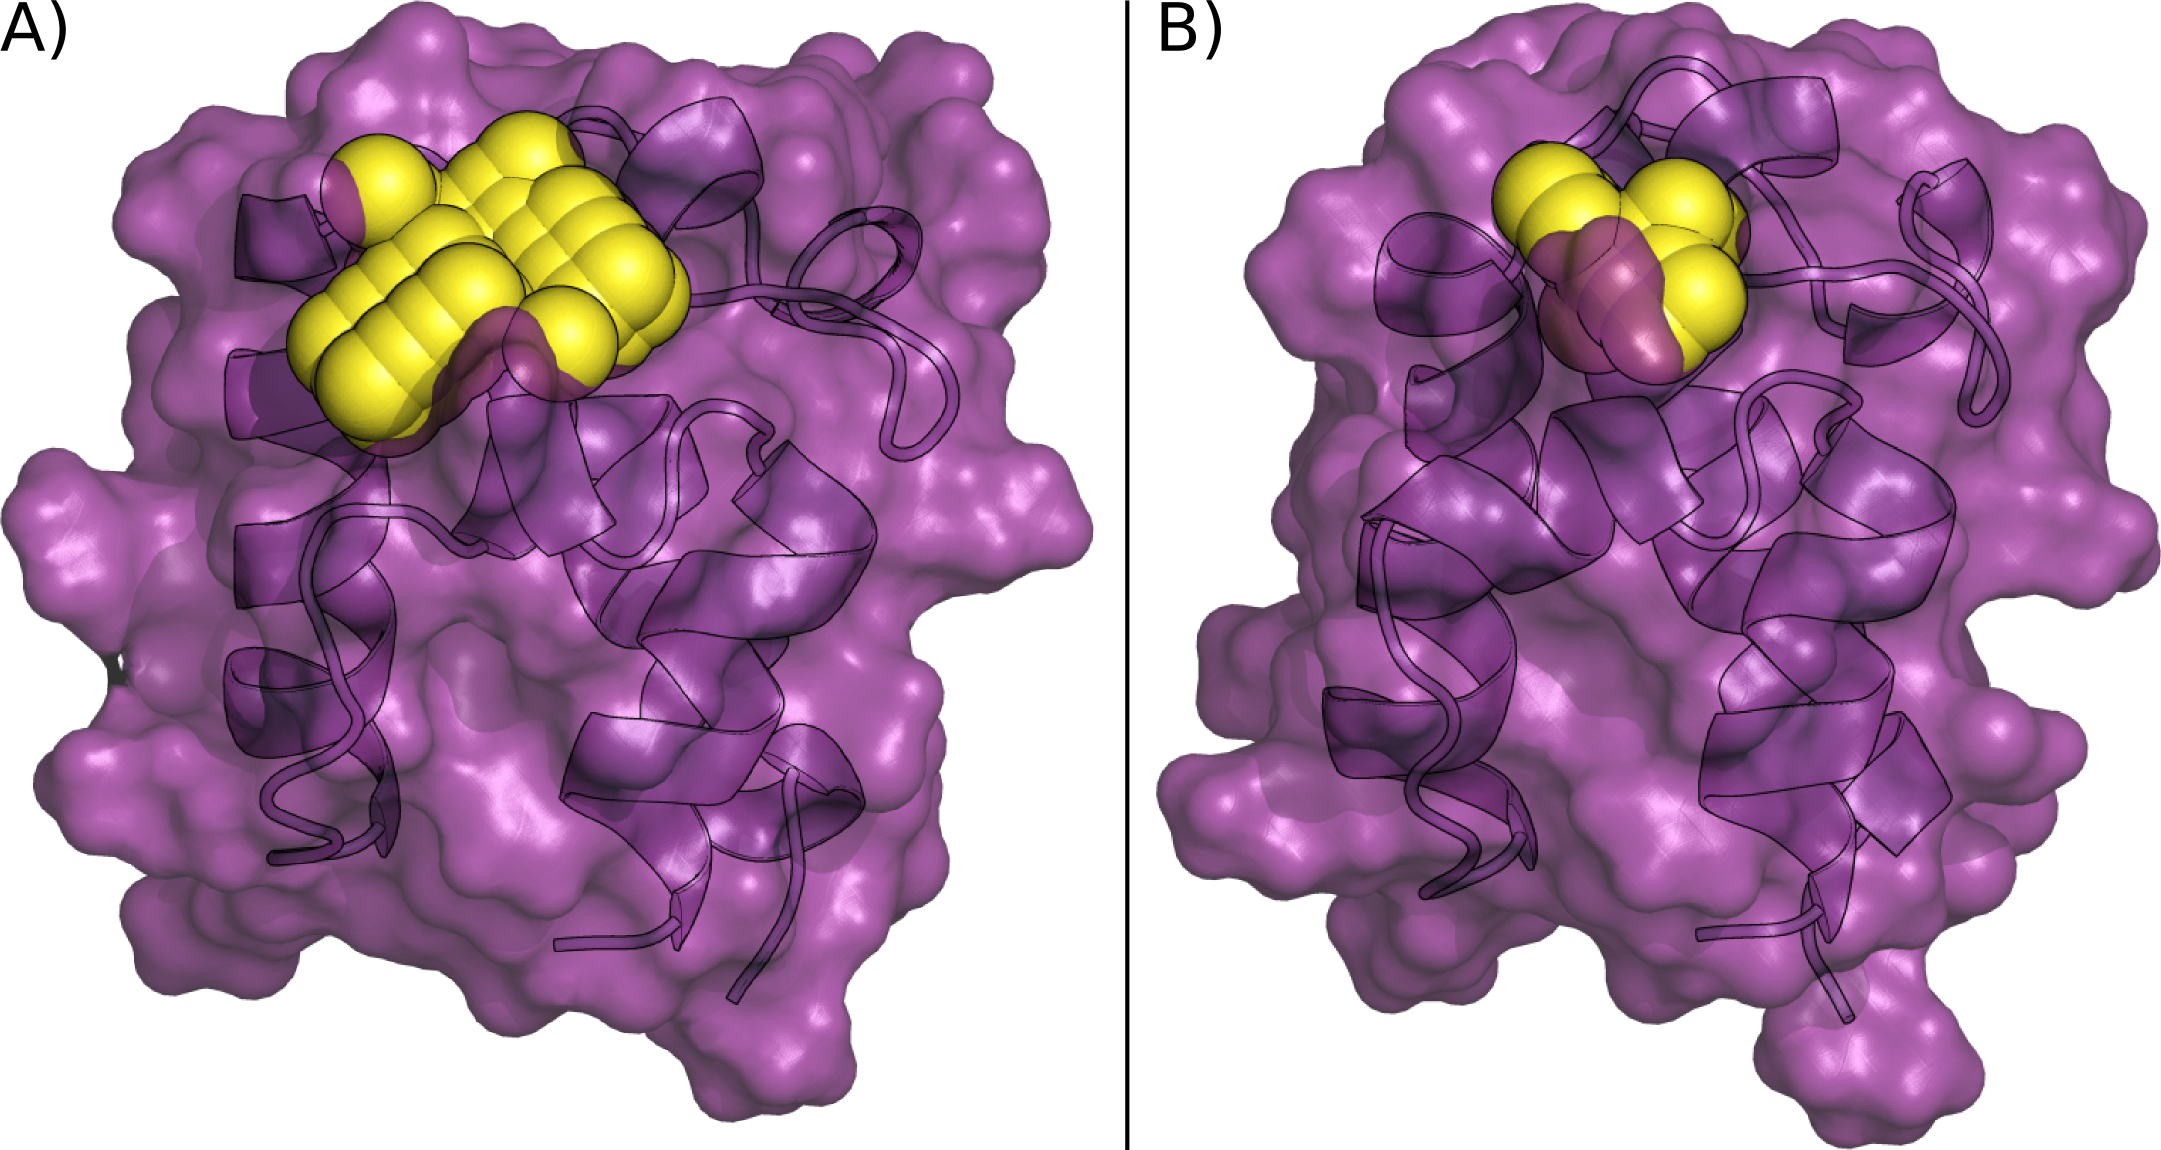
\includegraphics[width=0.9\textwidth, keepaspectratio=true]{graphics/acp_mutant.png}}
		\caption[Space filled diagram of the largest and the modal cavity volume in the apo ACP-mupA3a W44L.]{Space filled diagram of the largest (A) and the modal (B) cavity volume in the apo ACP-mupA3a W44L.}
		\label{fig:acp_mutant}
		\end{figure}		

		\setlength\fboxsep{5pt}
		\setlength\fboxrule{1.5pt}
		\begin{figure}[htbp]
		\centering
		\fbox{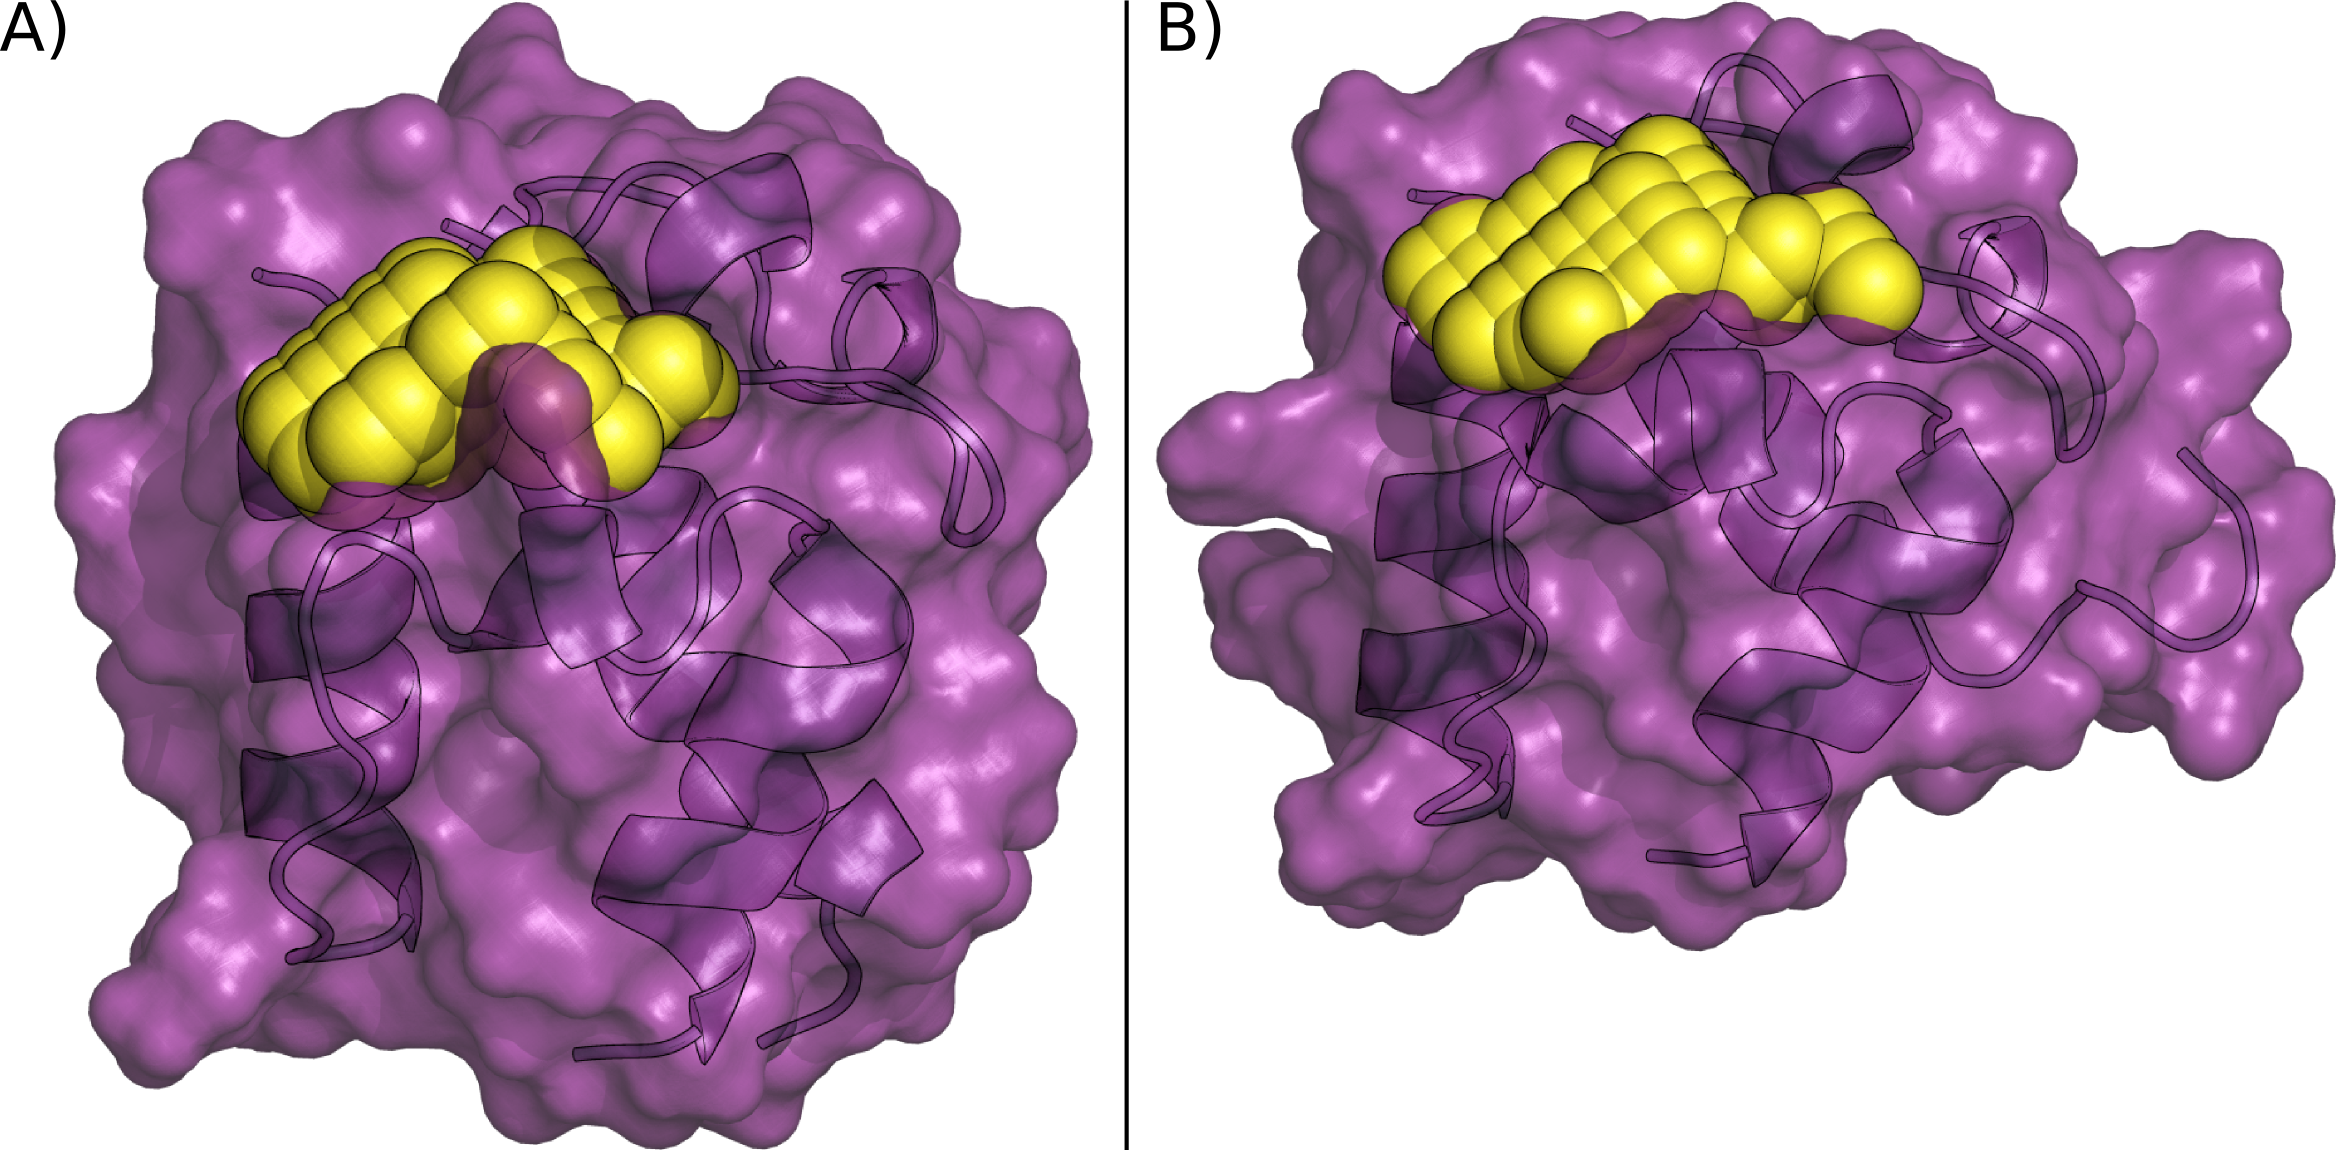
\includegraphics[width=0.9\textwidth, keepaspectratio=true]{graphics/ppt_wild.png}}
		\caption[Space filled diagram of the largest and the modal cavity volume in the holo ACP-mupA3a WT.]{Space filled diagram of the largest (A) and the modal (B) cavity volume in the holo ACP-mupA3a WT.}
		\label{fig:ppt_wild}
		\end{figure}


		\setlength\fboxsep{5pt}
		\setlength\fboxrule{1.5pt}
		\begin{figure}[htbp]
		\centering
		\fbox{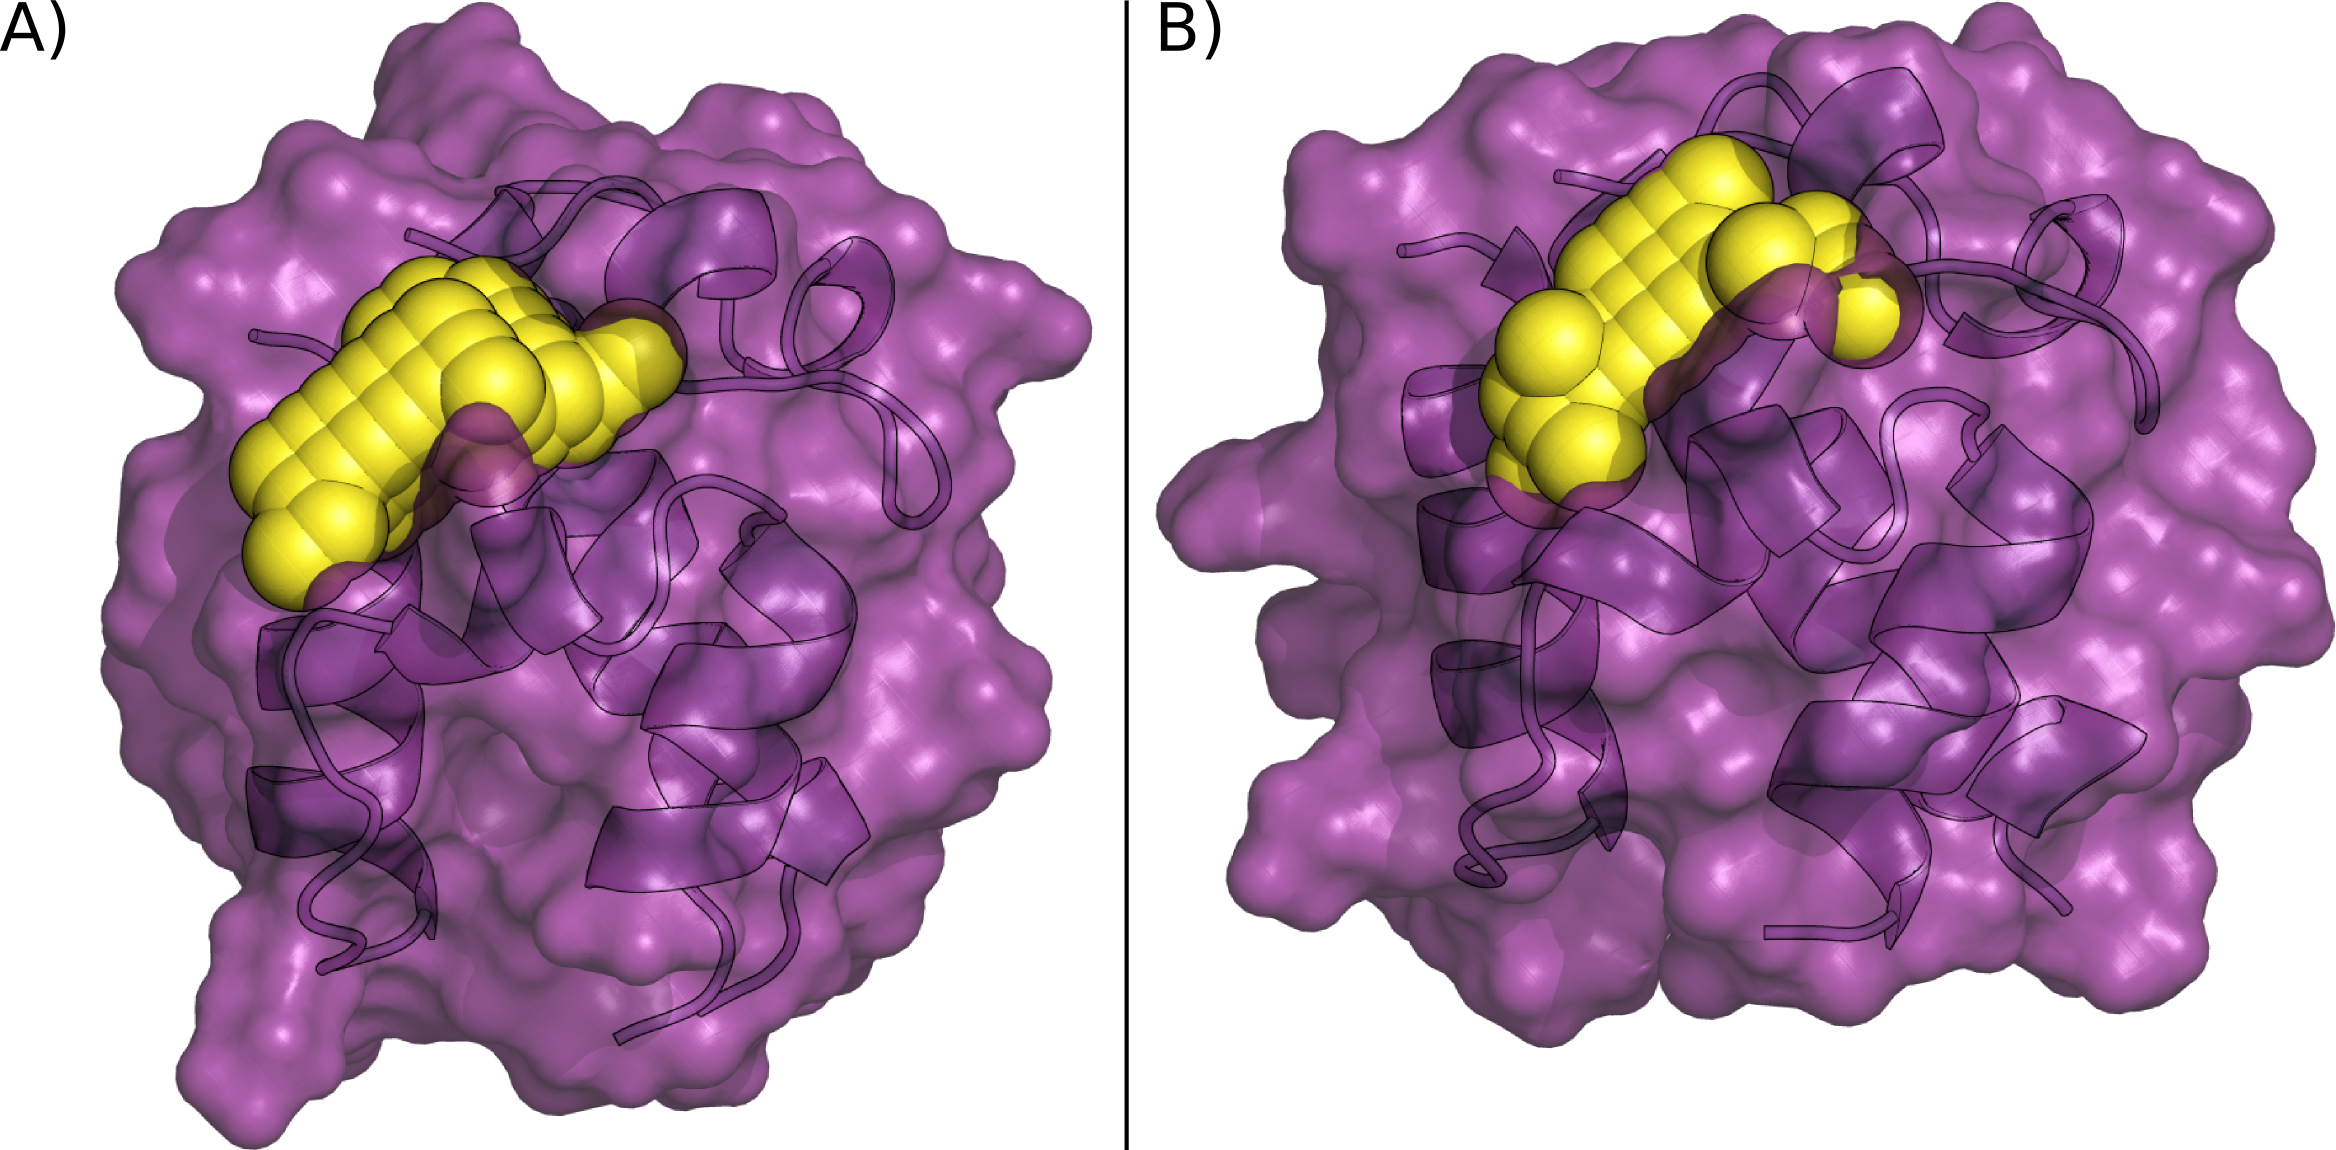
\includegraphics[width=0.9\textwidth, keepaspectratio=true]{graphics/ppt_mutant.png}}
		\caption[Space filled diagram of the largest and the modal cavity volume in the holo ACP-mupA3a W44L.]{Space filled diagram of the largest (A) and the modal (B) cavity volume in the holo ACP-mupA3a W44L.}
		\label{fig:ppt_mutant}
		\end{figure}

		\setlength\fboxsep{5pt}
		\setlength\fboxrule{1.5pt}
		\begin{figure}[htbp]
		\centering
		\fbox{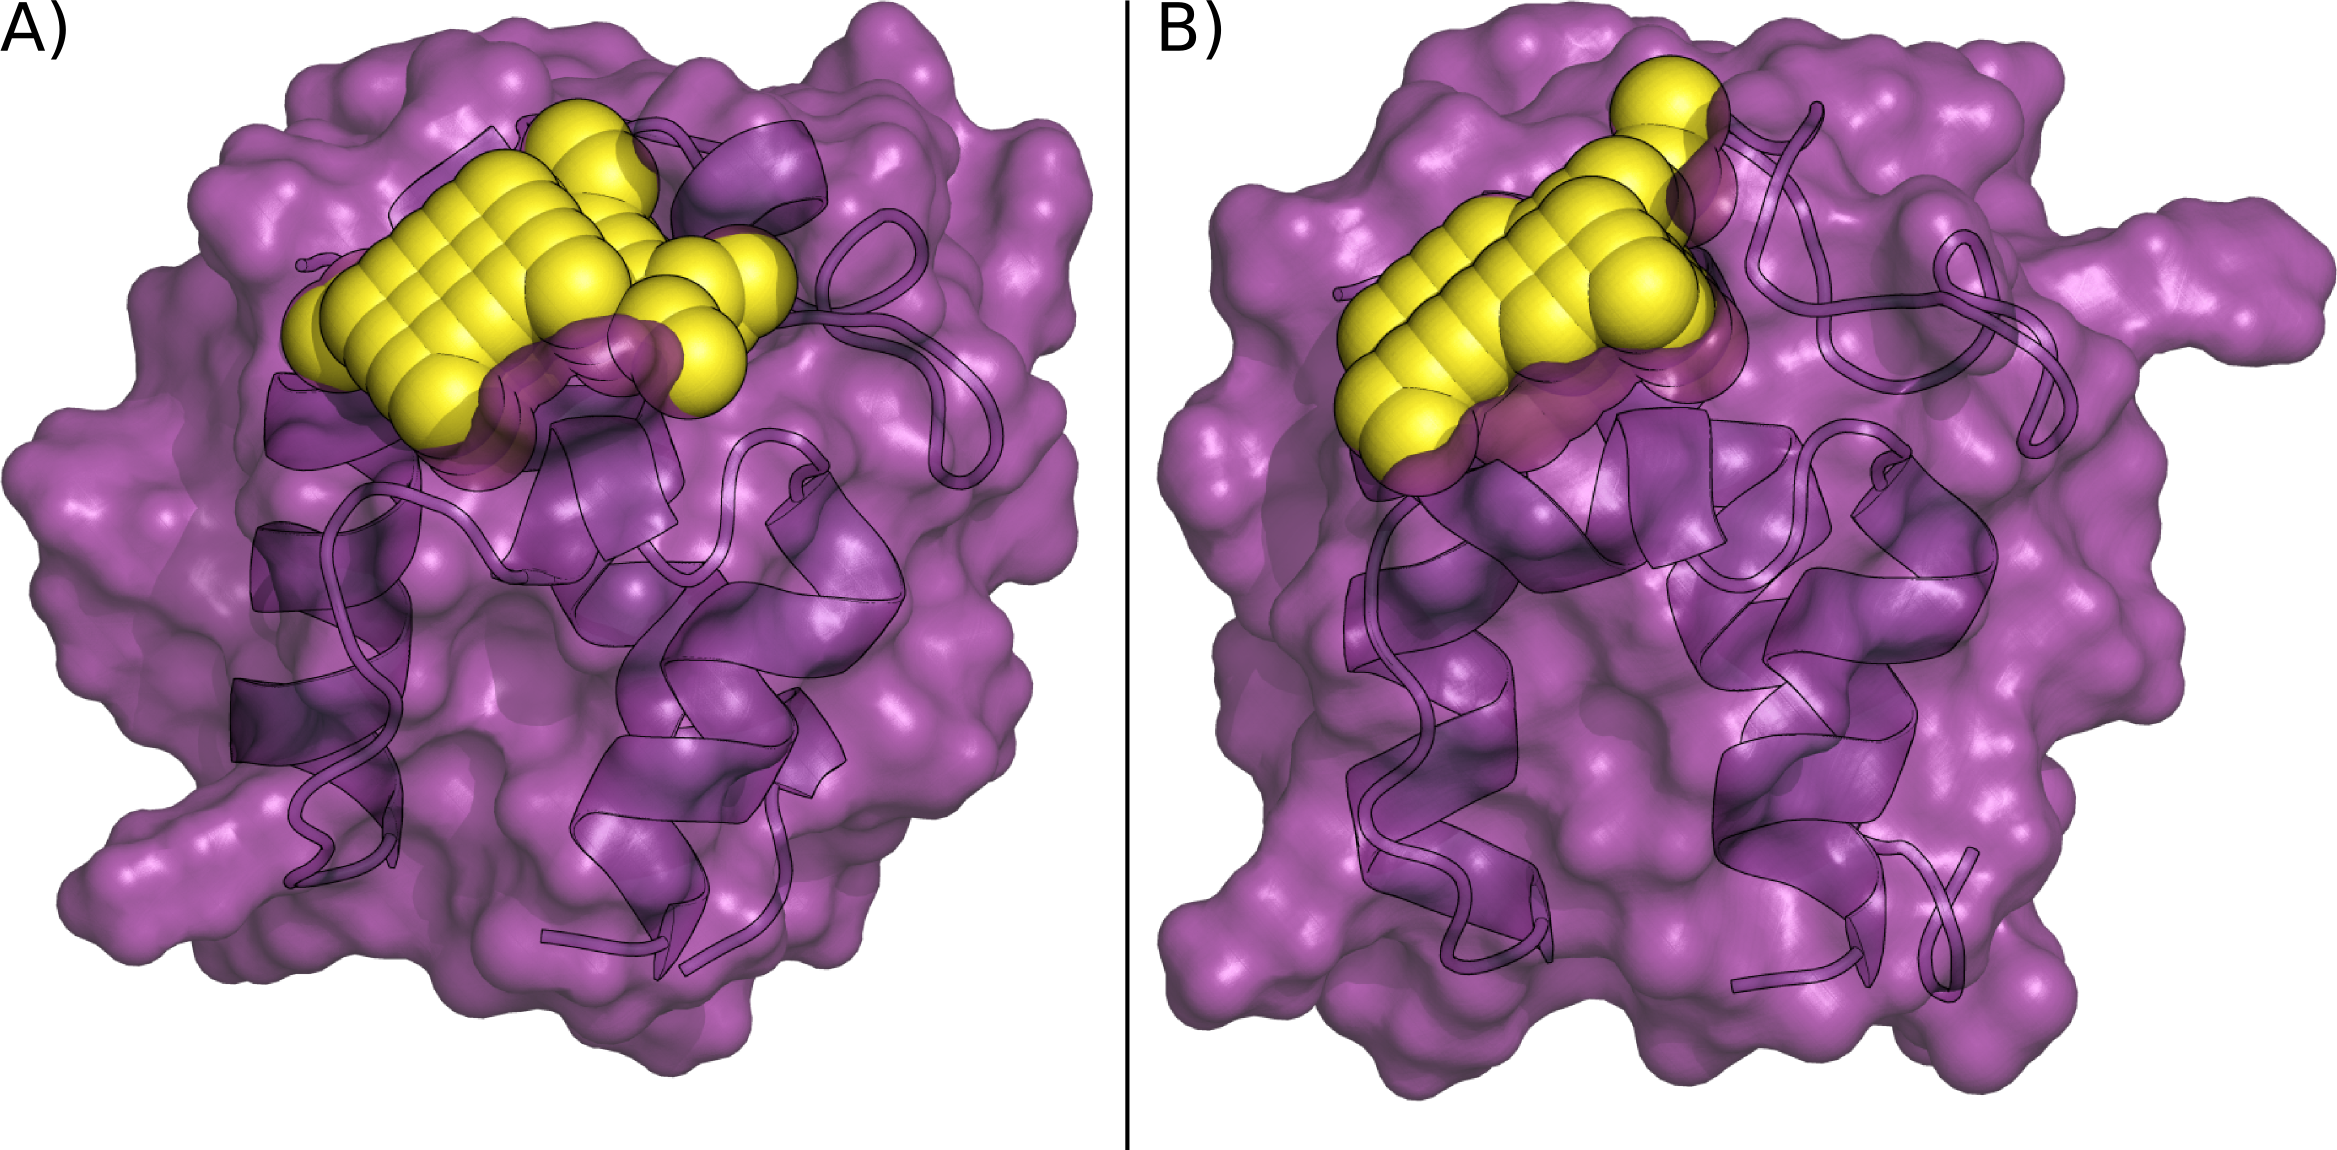
\includegraphics[width=0.9\textwidth, keepaspectratio=true]{graphics/spm_mutant.png}}
		\caption[Space filled diagram of the largest and the modal cavity volume in the acyl ACP-mupA3a W44L.]{Space filled diagram of the largest (A) and the modal (B) cavity volume in the acyl ACP-mupA3a W44L.}
		\label{fig:spm_mutant}
		\end{figure}

		\setlength\fboxsep{5pt}
		\setlength\fboxrule{1.5pt}
		\begin{figure}[htbp]
		\centering
		\fbox{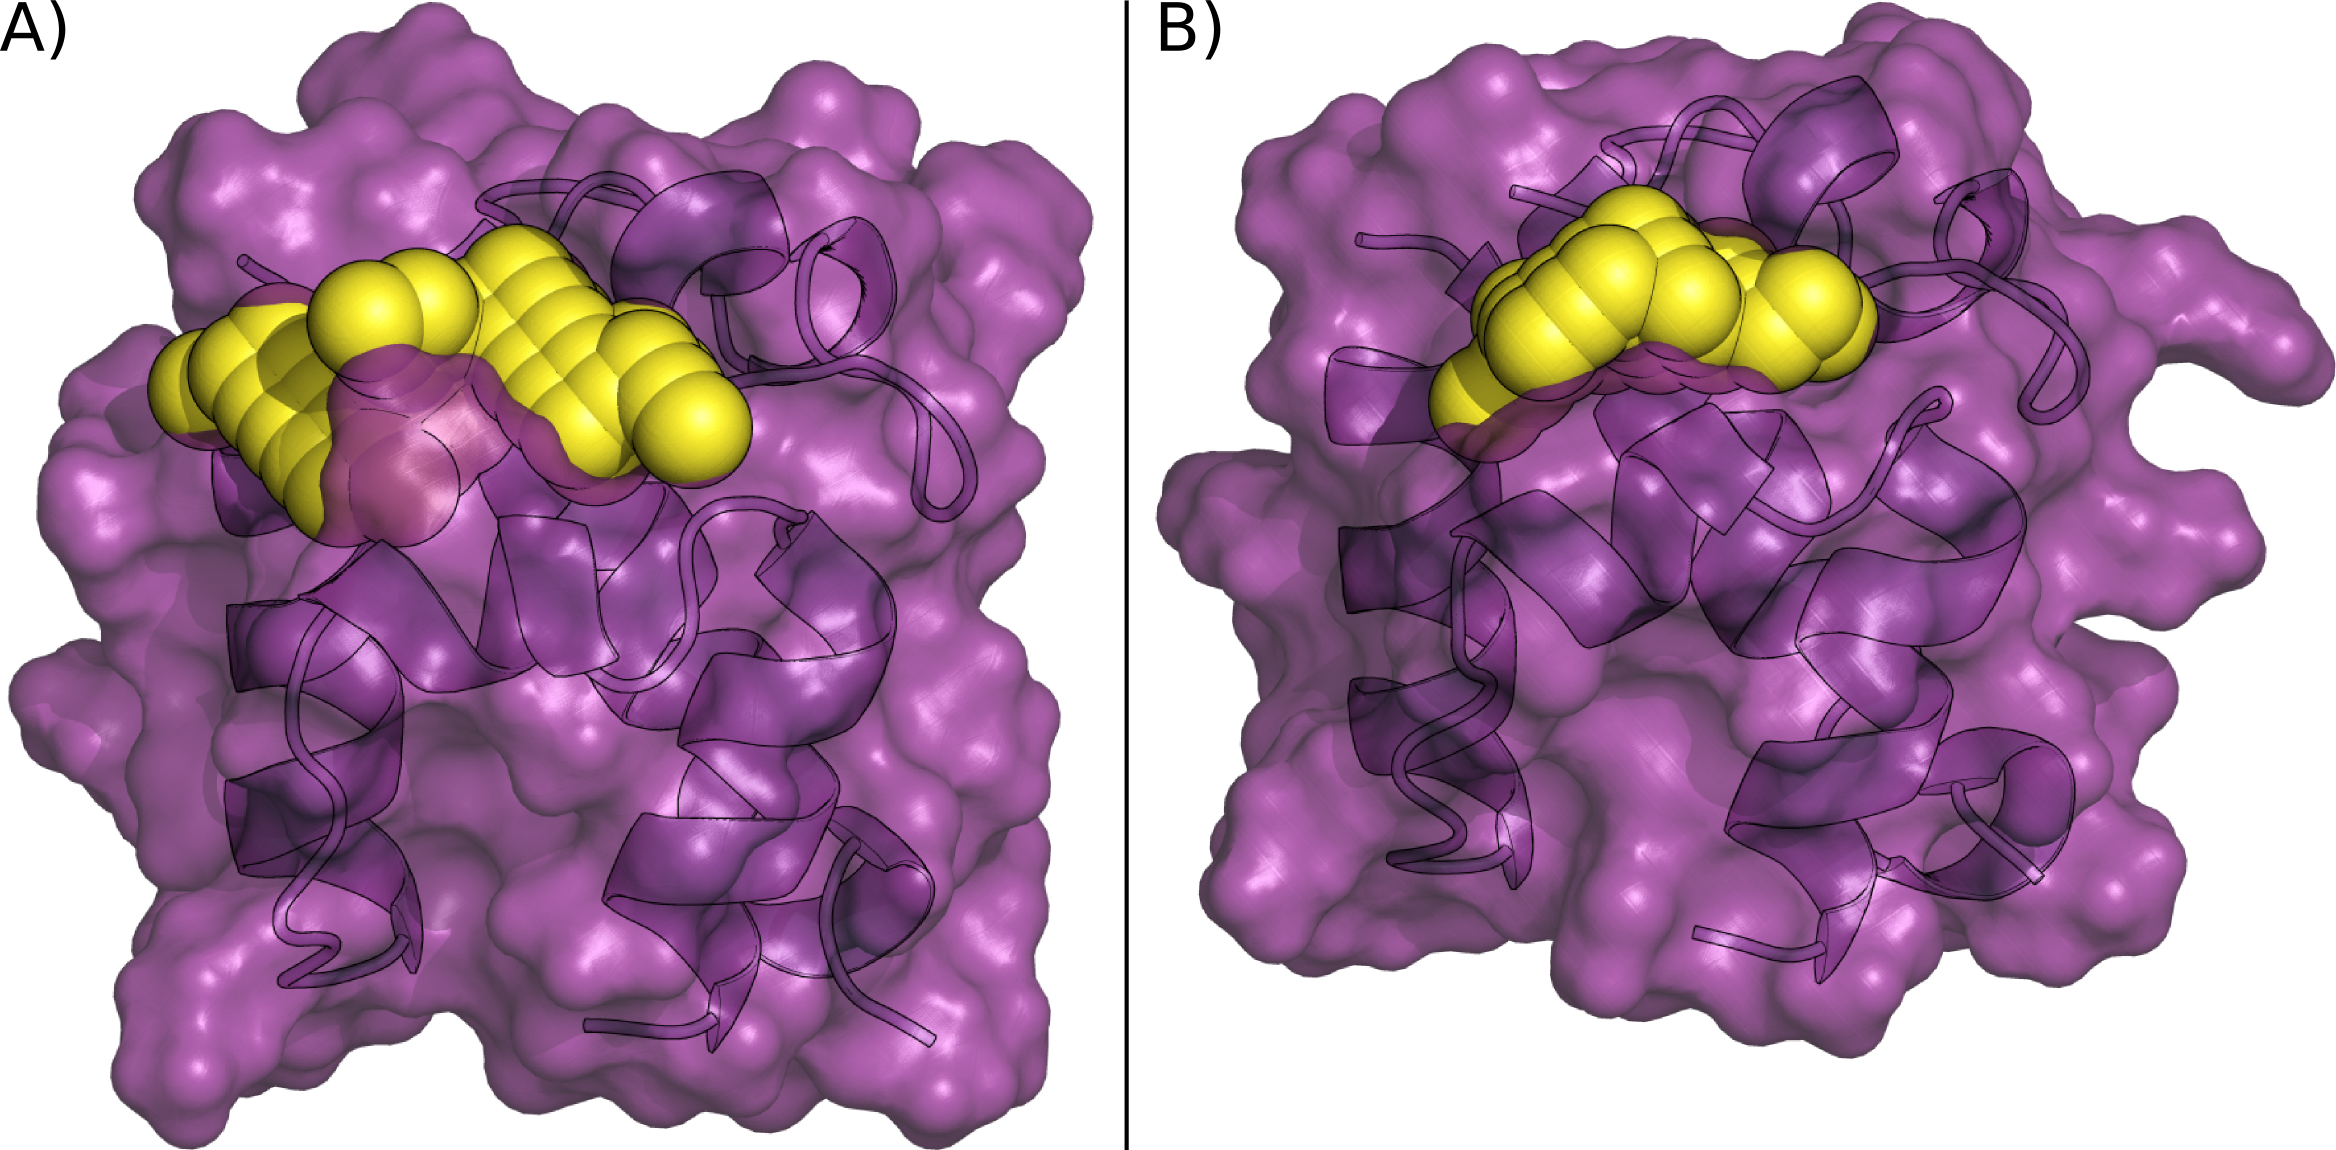
\includegraphics[width=0.9\textwidth, keepaspectratio=true]{graphics/spd.png}}
		\caption[Space filled diagram of the largest and the modal cavity volume in the acyl 14C ACP-mupA3a.]{Space filled diagram of the largest (A) and the modal (B) cavity volume in the acyl 14C ACP-mupA3a.}
		\label{fig:spd}
		\end{figure}

		\setlength\fboxsep{5pt}
		\setlength\fboxrule{1.5pt}
		\begin{figure}[htbp]
		\centering
		\fbox{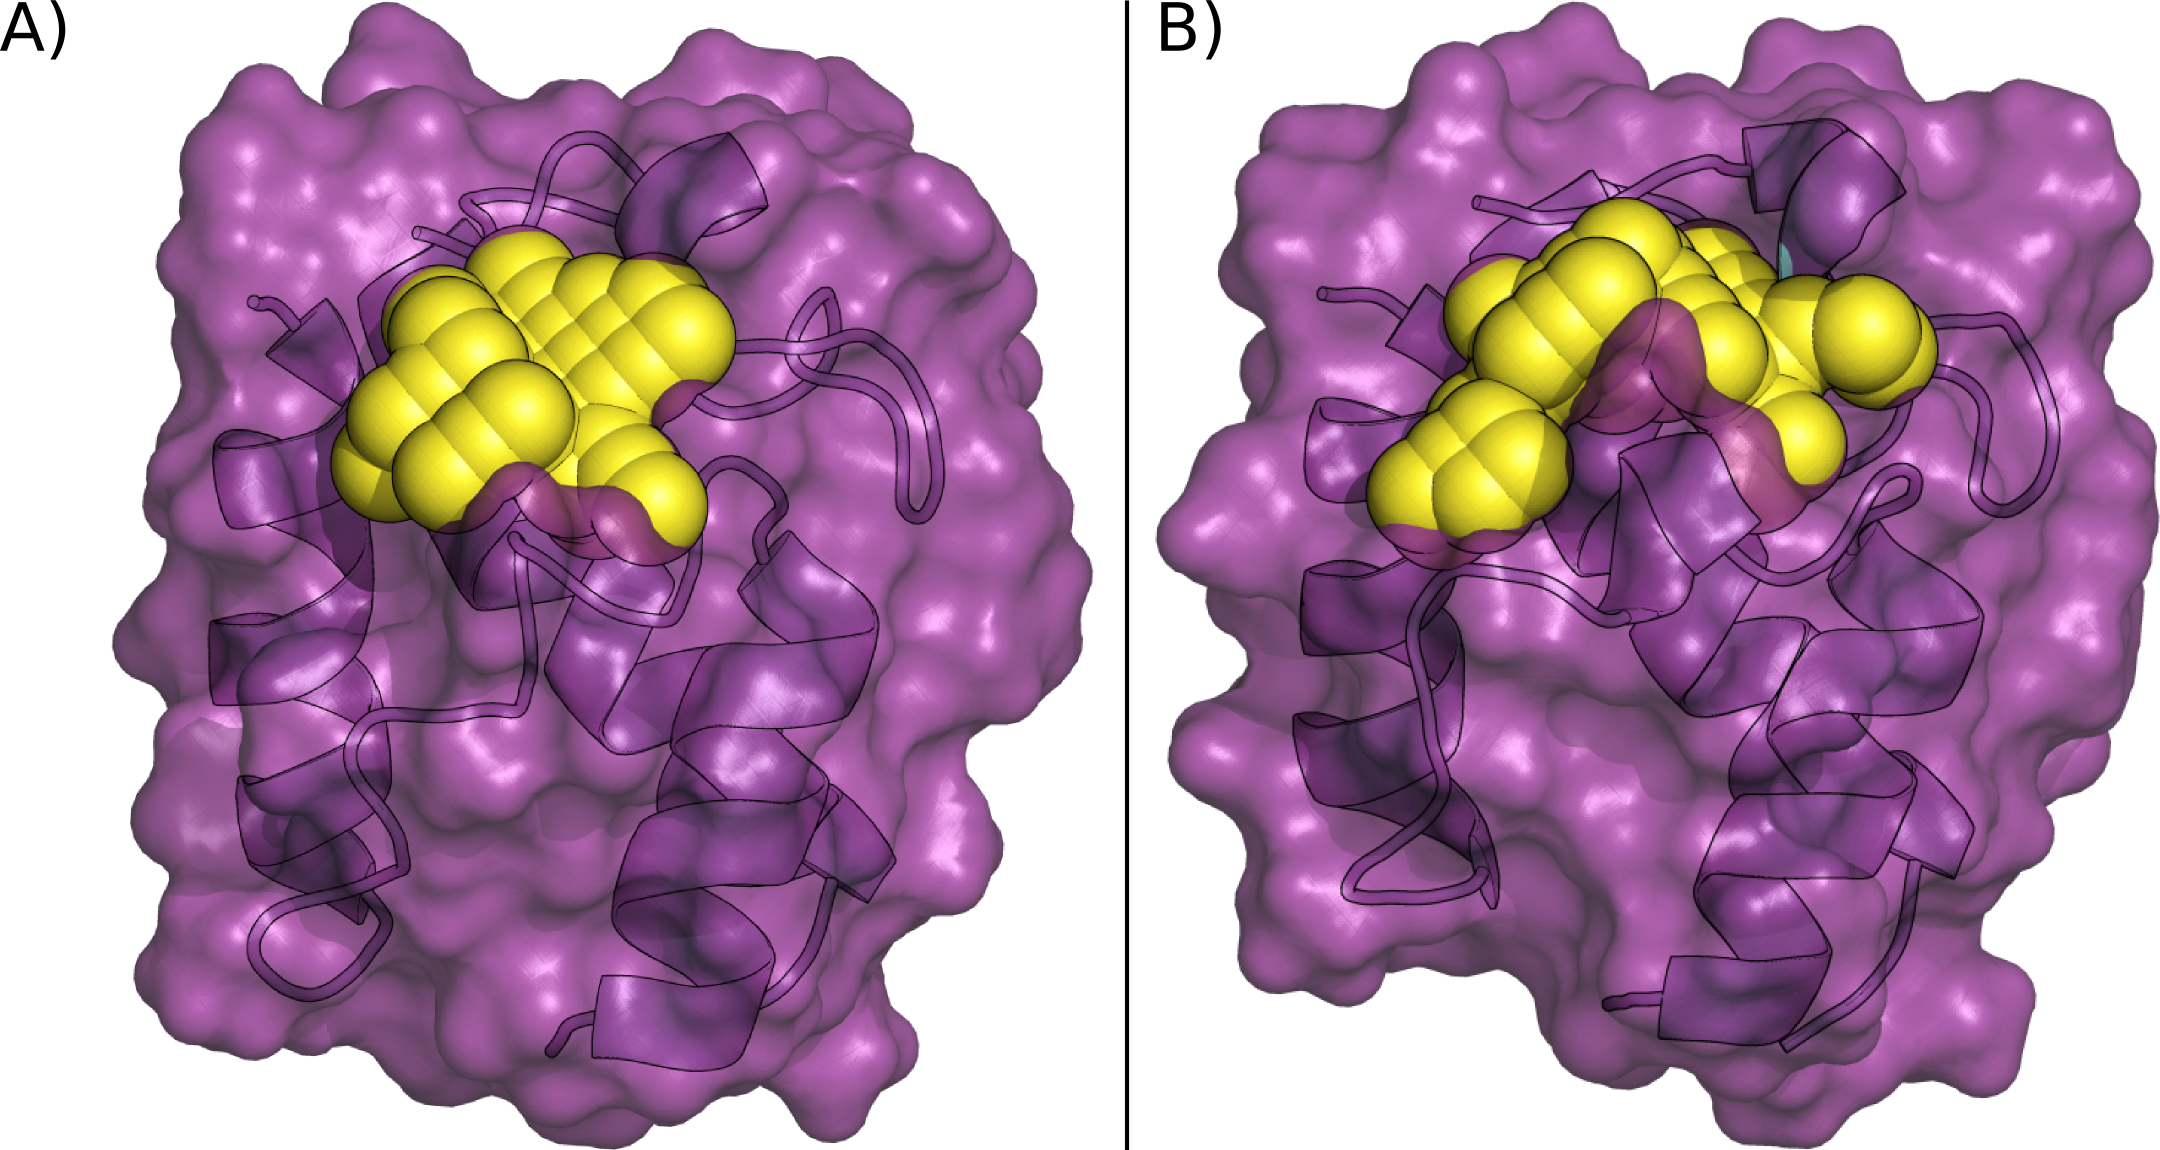
\includegraphics[width=0.9\textwidth, keepaspectratio=true]{graphics/acp2.png}}
		\caption[Space filled diagram of the largest and the modal cavity volume in the acyl ACP-mupA2a.]{Space filled diagram of the largest (A) and the modal (B) cavity volume in the acyl ACP-mupA2a.}
		\label{fig:acp2}
		\end{figure}

								
		
\newpage
	\subsection{Change in RMSD of PKS ACPs from FAS ACP over time}
	\label{sec:AppIII:rmsd}	
	
		\setlength\fboxsep{5pt}
		\setlength\fboxrule{1.5pt}
		\begin{figure}[htbp]
		\centering
		\fbox{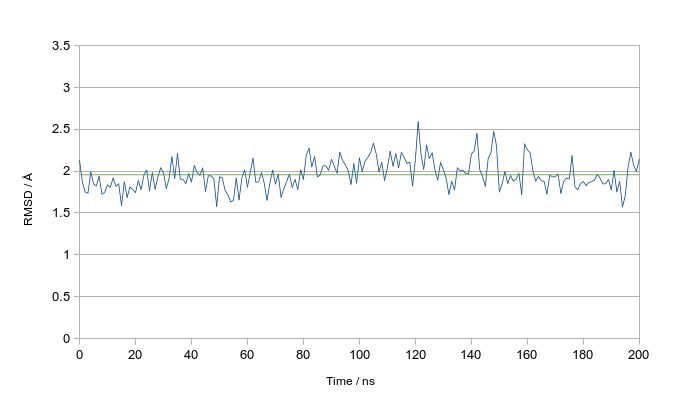
\includegraphics[width=0.9\textwidth, keepaspectratio=true]{graphics/RmsdAcpWild.png}}
		\caption[RMSD between FAS ACP and apo ACP-mupA3a WT over time (200 ns).]{RMSD between FAS ACP and apo ACP-mupA3a WT over time (200 ns). Green line represents the mean.}
		\label{fig:RmsdAcpWild}
		\end{figure}	

		\setlength\fboxsep{5pt}
		\setlength\fboxrule{1.5pt}
		\begin{figure}[htbp]
		\centering
		\fbox{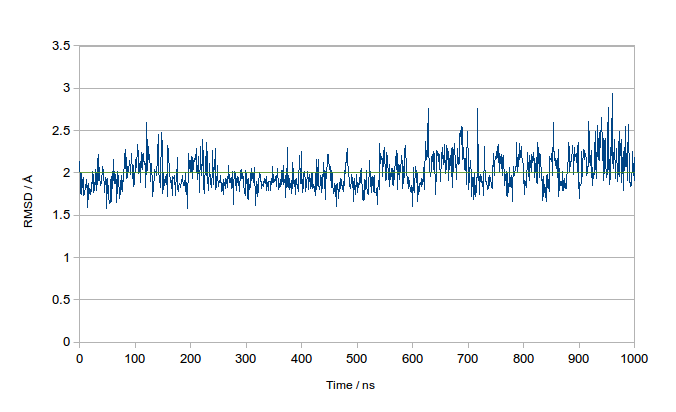
\includegraphics[width=0.9\textwidth, keepaspectratio=true]{graphics/RmsdAcpWild_1000.png}}
		\caption[RMSD between FAS ACP and apo ACP-mupA3a WT over time (1 $ \mu $s).]{RMSD between FAS ACP and apo ACP-mupA3a WT over time (1 $ \mu $s). Green line represents the mean.}
		\label{fig:RmsdAcpWild_1000}
		\end{figure}	
		
		\setlength\fboxsep{5pt}
		\setlength\fboxrule{1.5pt}
		\begin{figure}[htbp]
		\centering
		\fbox{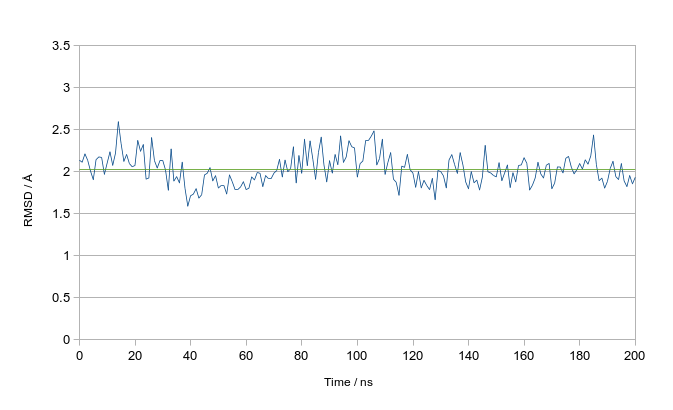
\includegraphics[width=0.9\textwidth, keepaspectratio=true]{graphics/RmsdAcpMutant.png}}
		\caption[RMSD between FAS ACP and apo ACP-mupA3a W44L over time.]{RMSD between FAS ACP and apo ACP-mupA3a W44L over time. Green line represents the mean.}
		\label{fig:RmsdAcpMutant}
		\end{figure}	

		\setlength\fboxsep{5pt}
		\setlength\fboxrule{1.5pt}
		\begin{figure}[htbp]
		\centering
		\fbox{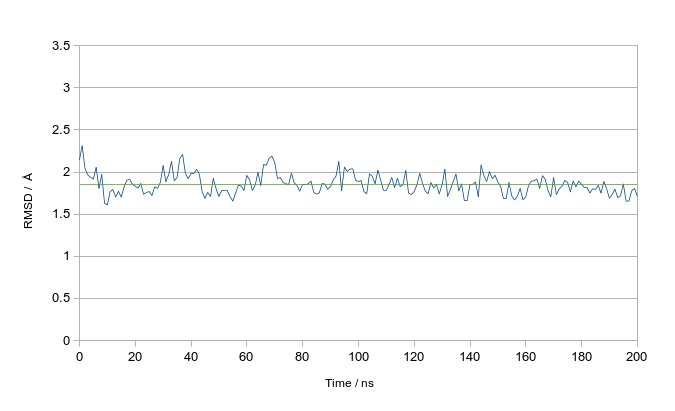
\includegraphics[width=0.9\textwidth, keepaspectratio=true]{graphics/RmsdAcpPPTWild.png}}
		\caption[RMSD between FAS ACP and the holo ACP-mupA3a WT over time.]{RMSD between FAS ACP and the holo ACP-mupA3a WT over time. Green line represents the mean.}
		\label{fig:RmsdAcpPPTWild}
		\end{figure}

		\setlength\fboxsep{5pt}
		\setlength\fboxrule{1.5pt}
		\begin{figure}[htbp]
		\centering
		\fbox{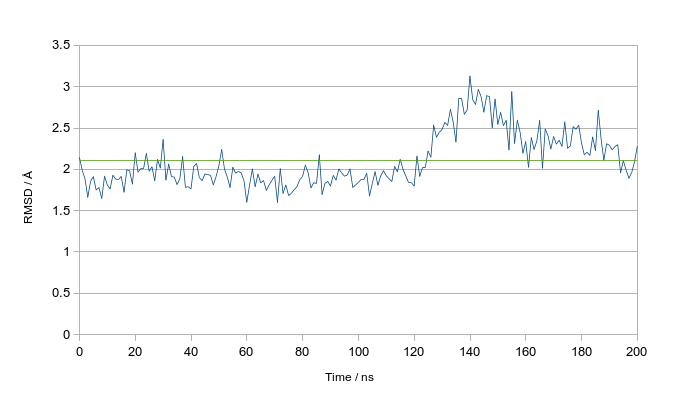
\includegraphics[width=0.9\textwidth, keepaspectratio=true]{graphics/RmsdAcpPPTMutant.png}}
		\caption[RMSD between FAS ACP and the holo ACP-mupA3a W44L over time.]{RMSD between FAS ACP and the holo ACP-mupA3a W44L over time. Green line represents the mean.}
		\label{fig:RmsdAcpPPTMutant}
		\end{figure}
		
		\setlength\fboxsep{5pt}
		\setlength\fboxrule{1.5pt}
		\begin{figure}[htbp]
		\centering
		\fbox{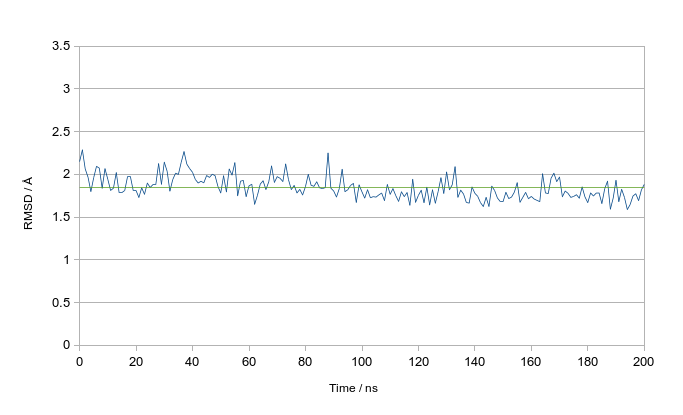
\includegraphics[width=0.9\textwidth, keepaspectratio=true]{graphics/RMSDACPSPMWild_200.png}}
		\caption[RMSD between FAS ACP and the acyl ACP-mupA3a WT over time (200 ns).]{RMSD between FAS ACP and the acyl ACP-mupA3a WT over time (200 ns). Green line represents the mean.}
		\label{fig:RMSDACPSPMWild_200}
		\end{figure}

		\setlength\fboxsep{5pt}
		\setlength\fboxrule{1.5pt}
		\begin{figure}[htbp]
		\centering
		\fbox{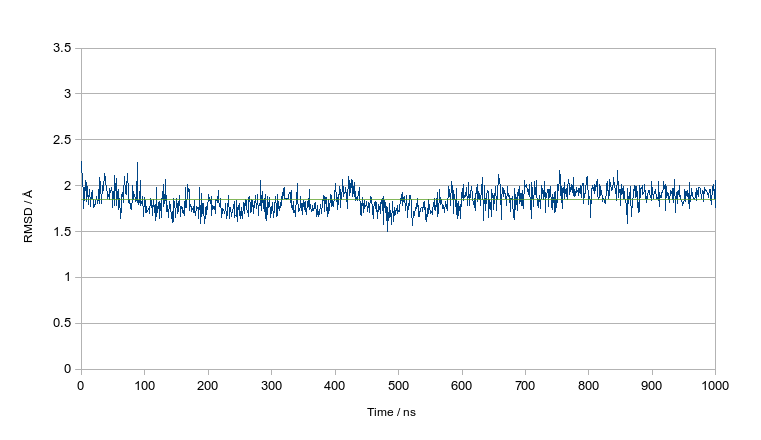
\includegraphics[width=0.9\textwidth, keepaspectratio=true]{graphics/RMSDACPSPMWild_1000.png}}
		\caption[RMSD between FAS ACP and the acyl ACP-mupA3a WT over time (1 $ \mu $s).]{RMSD between FAS ACP and the acyl ACP-mupA3a WT over time (1 $ \mu $s). Green line represents the mean.}
		\label{fig:RMSDACPSPMWild_1000}
		\end{figure}		

		\setlength\fboxsep{5pt}
		\setlength\fboxrule{1.5pt}
		\begin{figure}[htbp]
		\centering
		\fbox{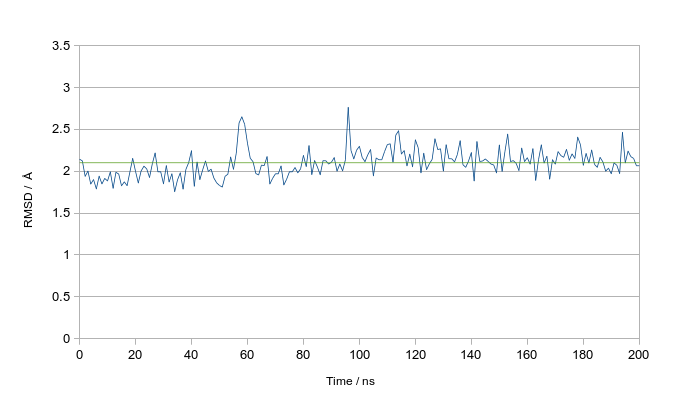
\includegraphics[width=0.9\textwidth, keepaspectratio=true]{graphics/RMSDACPSPMMutant_200.png}}
		\caption[RMSD between FAS ACP and the acyl ACP-mupA3a W44L over time.]{RMSD between FAS ACP and the acyl ACP-mupA3a W44L over time. Green line represents the mean.}
		\label{fig:RMSDACPSPMMutant_200}
		\end{figure}		


		\setlength\fboxsep{5pt}
		\setlength\fboxrule{1.5pt}
		\begin{figure}[htbp]
		\centering
		\fbox{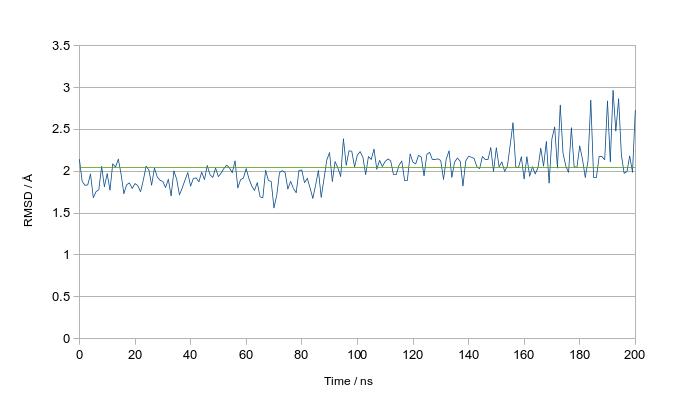
\includegraphics[width=0.9\textwidth, keepaspectratio=true]{graphics/RmsdACPSPD.png}}
		\caption[RMSD between FAS ACP and the acyl 14C ACP-mupA3a over time.]{RMSD between FAS ACP and the acyl 14C ACP-mupA3a over time. Green line represents the mean.}
		\label{fig:RmsdACPSPD}
		\end{figure}

		\setlength\fboxsep{5pt}
		\setlength\fboxrule{1.5pt}
		\begin{figure}[htbp]
		\centering
		\fbox{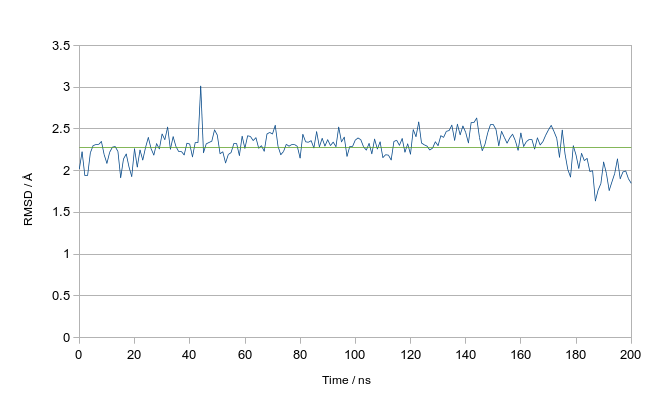
\includegraphics[width=0.9\textwidth, keepaspectratio=true]{graphics/RmsdACP2.png}}
		\caption[RMSD between FAS ACP and the acyl ACP-mupA2a over time.]{RMSD between FAS ACP and the acyl ACP-mupA2a over time. Green line represents the mean.}
		\label{fig:RmsdACP2}
		\end{figure}

\newpage
	\subsection{Hydrogen bonding between the phosphopantetheine, acyl groups and protein/solvent}
	\label{sec:AppIII:hb}

		\setlength\fboxsep{5pt}
		\setlength\fboxrule{1.5pt}
		\begin{figure}[htbp]
		\centering
		\fbox{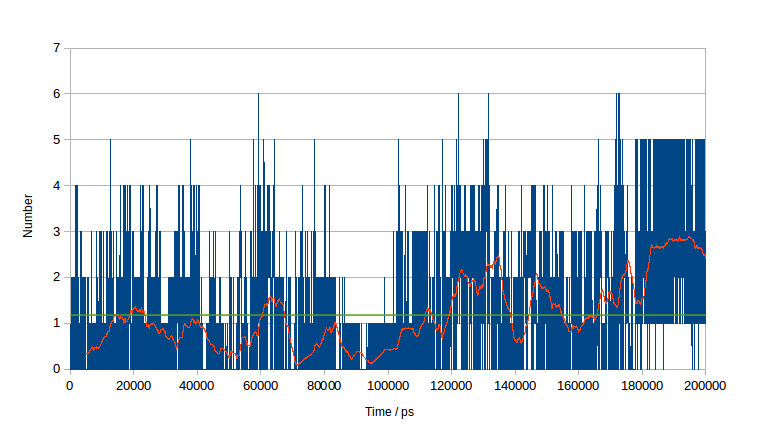
\includegraphics[width=0.9\textwidth, keepaspectratio=true]{graphics/HbondACPPPTWild_protein.png}}
		\caption[Number of hydrogen bonds formed between the phosphopantetheine and the ACP-mupA3a WT surface residues.]{Number of hydrogen bonds formed between the phosphopantetheine and the ACP-mupA3a WT surface residues.  Red line represents the running average over 500 frames and green line represents the mean.}
		\label{fig:HbondACPPPTWild_protein}
		\end{figure}

		\setlength\fboxsep{5pt}
		\setlength\fboxrule{1.5pt}
		\begin{figure}[htbp]
		\centering
		\fbox{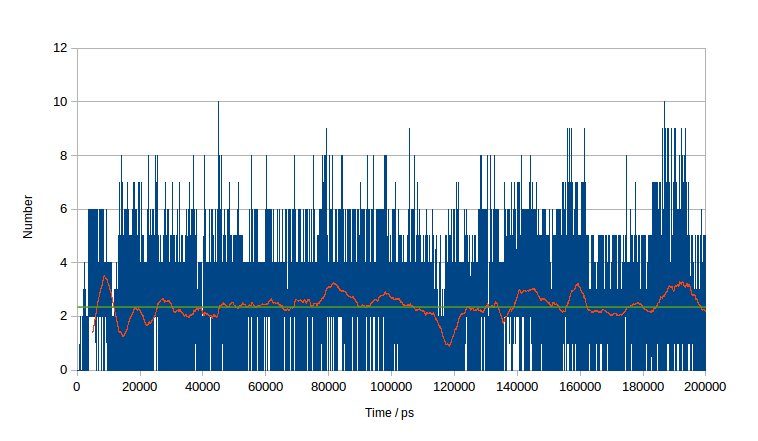
\includegraphics[width=0.9\textwidth, keepaspectratio=true]{graphics/HbondACPPPTMutant_protein.png}}
		\caption[Number of hydrogen bonds formed between the phosphopantetheine and the ACP-mupA3a W44L surface residues.]{Number of hydrogen bonds formed between the phosphopantetheine and the ACP-mupA3a W44L surface residues.  Red line represents the running average over 500 frames and green line represents the mean.}
		\label{fig:HbondACPPPTMutant_protein}
		\end{figure}

		\setlength\fboxsep{5pt}
		\setlength\fboxrule{1.5pt}
		\begin{figure}[htbp]
		\centering
		\fbox{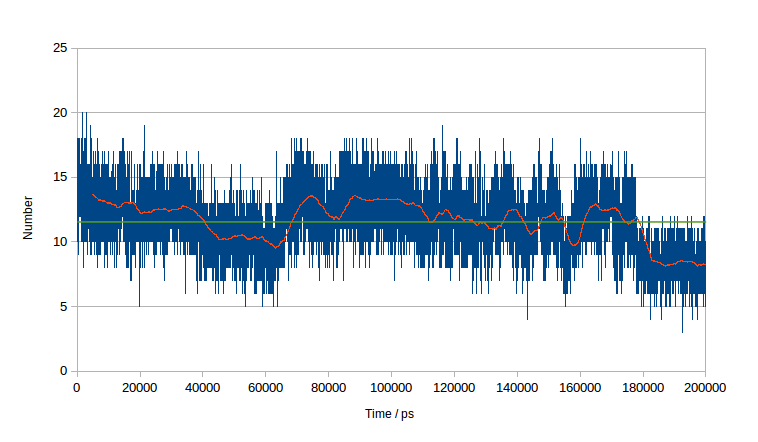
\includegraphics[width=0.9\textwidth, keepaspectratio=true]{graphics/HbondACPPPTWild_solvent.png}}
		\caption[Number of hydrogen bonds formed between the phosphopantetheine and the solvent in the ACP-mupA3a WT.]{Number of hydrogen bonds formed between the phosphopantetheine and the solvent in the ACP-mupA3a WT.  Red line represents the running average over 500 frames and green line represents the mean.}
		\label{fig:HbondACPPPTWild_solvent}
		\end{figure}	
		
		\setlength\fboxsep{5pt}
		\setlength\fboxrule{1.5pt}
		\begin{figure}[htbp]
		\centering
		\fbox{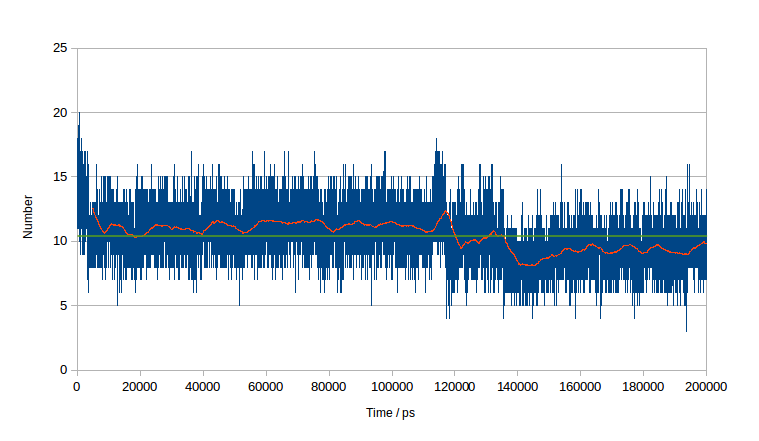
\includegraphics[width=0.9\textwidth, keepaspectratio=true]{graphics/HbondACPPPTMutant_solvent.png}}
		\caption[Number of hydrogen bonds formed between the phosphopantetheine and the solvent in the ACP-mupA3a W44L.]{Number of hydrogen bonds formed between the phosphopantetheine and the solvent in the ACP-mupA3a W44L.  Red line represents the running average over 500 frames and green line represents the mean.}
		\label{fig:HbondACPPPTMutant_solvent}
		\end{figure}	


		\setlength\fboxsep{5pt}
		\setlength\fboxrule{1.5pt}
		\begin{figure}[htbp]
		\centering
		\fbox{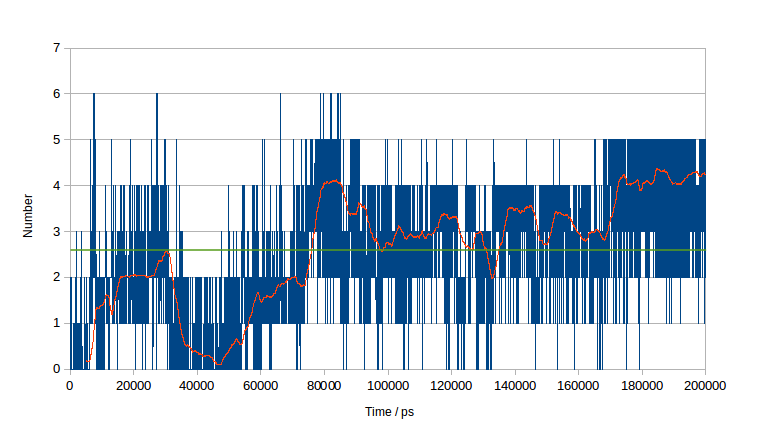
\includegraphics[width=0.9\textwidth, keepaspectratio=true]{graphics/HbondACPSPMWild200_protein.png}}
		\caption[Number of hydrogen bonds formed between the ACP-mupA3a cognate substrate and the ACP-mupA3a WT surface residues over time (200 ns).]{Number of hydrogen bonds formed between the ACP-mupA3a cognate substrate and the ACP-mupA3a WT surface residues over time (200 ns).  Red line represents the running average over 500 frames and green line represents the mean.}
		\label{fig:HbondACPSPMWild200_protein}
		\end{figure}

		\setlength\fboxsep{5pt}
		\setlength\fboxrule{1.5pt}
		\begin{figure}[htbp]
		\centering
		\fbox{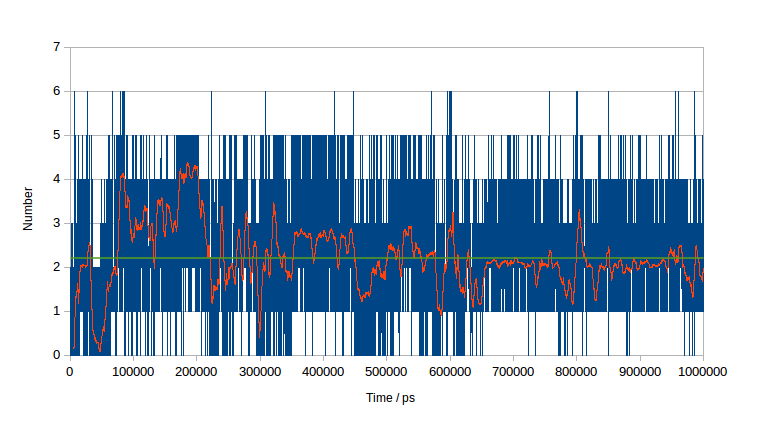
\includegraphics[width=0.9\textwidth, keepaspectratio=true]{graphics/HbondACPSPMWild1000_protein.png}}
		\caption[Number of hydrogen bonds formed between the ACP-mupA3a cognate substrate and the ACP-mupA3a WT surface residues over time (1 $ \mu $s).]{Number of hydrogen bonds formed between the ACP-mupA3a cognate substrate and the ACP-mupA3a WT surface residues over time (1 $ \mu $s).  Red line represents the running average over 500 frames and green line represents the mean.}
		\label{fig:HbondACPSPMWild1000_protein}
		\end{figure}

		\setlength\fboxsep{5pt}
		\setlength\fboxrule{1.5pt}
		\begin{figure}[htbp]
		\centering
		\fbox{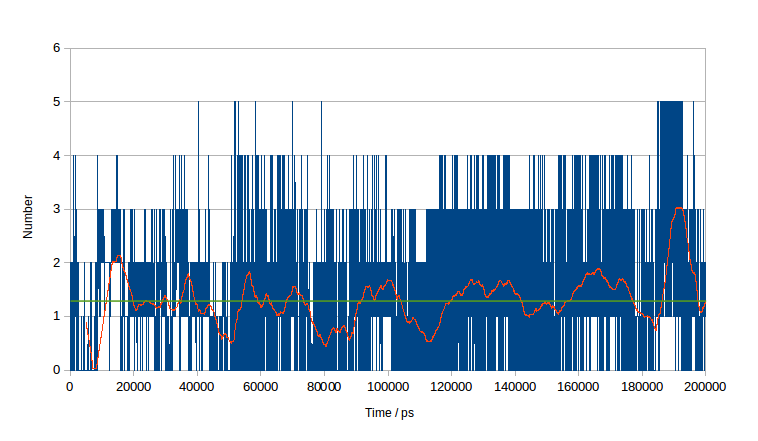
\includegraphics[width=0.9\textwidth, keepaspectratio=true]{graphics/HbondACPSPMMutant_protein.png}}
		\caption[Number of hydrogen bonds formed between the phosphopantetheine and the ACP-mupA3a W44L surface residues over time.]{Number of hydrogen bonds formed between the phosphopantetheine and the ACP-mupA3a W44L surface residues over time.  Red line represents the running average over 500 frames and green line represents the mean.}
		\label{fig:HbondACPSPMMutant_protein}
		\end{figure}

		\setlength\fboxsep{5pt}
		\setlength\fboxrule{1.5pt}
		\begin{figure}[htbp]
		\centering
		\fbox{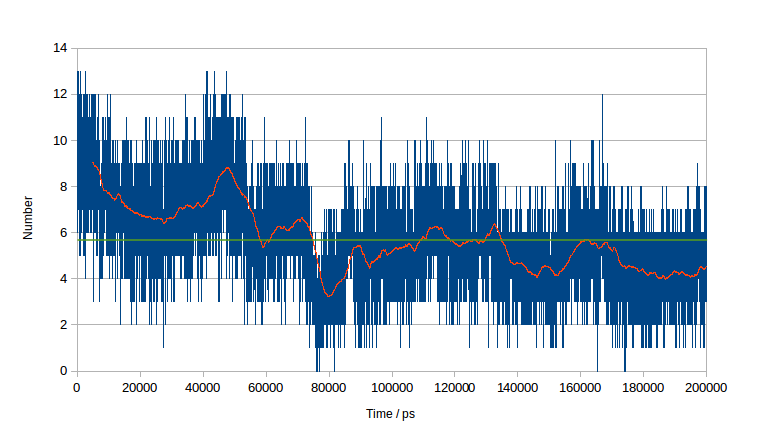
\includegraphics[width=0.9\textwidth, keepaspectratio=true]{graphics/HbondACPSPMWild200_solvent.png}}
		\caption[Number of hydrogen bonds formed between the ACP-mupA3a cognate substrate and the solvent in the acyl ACP-mupA3a WT simulation (200 ns).]{Number of hydrogen bonds formed between the ACP-mupA3a cognate substrate and the solvent in the acyl ACP-mupA3a WT simulation (200 ns).  Red line represents the running average over 500 frames and green line represents the mean.}
		\label{fig:HbondACPSPMWild200_solvent}
		\end{figure}

		\setlength\fboxsep{5pt}
		\setlength\fboxrule{1.5pt}
		\begin{figure}[htbp]
		\centering
		\fbox{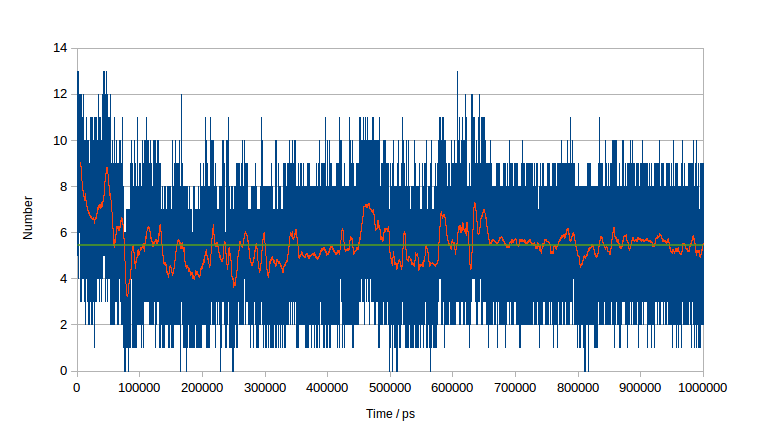
\includegraphics[width=0.9\textwidth, keepaspectratio=true]{graphics/HbondACPSPMWild1000_solvent.png}}
		\caption[Number of hydrogen bonds formed between the ACP-mupA3a cognate substrate and the solvent in the acyl ACP-mupA3a WT simulation (1 $ \mu $s).]{Number of hydrogen bonds formed between the ACP-mupA3a cognate substrate and the solvent in the acyl ACP-mupA3a WT simulation (1 $ \mu $s).  Red line represents the running average over 500 frames and green line represents the mean.}
		\label{fig:HbondACPSPMWild1000_solvent}
		\end{figure}			
		
		\setlength\fboxsep{5pt}
		\setlength\fboxrule{1.5pt}
		\begin{figure}[htbp]
		\centering
		\fbox{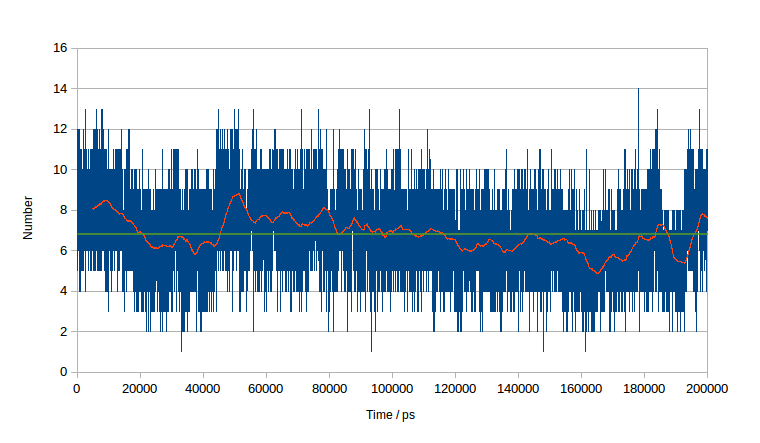
\includegraphics[width=0.9\textwidth, keepaspectratio=true]{graphics/HbondACPSPMMutant_solvent.png}}
		\caption[Number of hydrogen bonds formed between the ACP-mupA3a cognate substrate and the solvent in the acyl ACP-mupA3a W44L simulation.]{Number of hydrogen bonds formed between the ACP-mupA3a cognate substrate and the solvent in the acyl ACP-mupA3a W44L simulation.  Red line represents the running average over 500 frames and green line represents the mean.}
		\label{fig:HbondACPSPMMutant_solvent}
		\end{figure}	

		\setlength\fboxsep{5pt}
		\setlength\fboxrule{1.5pt}
		\begin{figure}[htbp]
		\centering
		\fbox{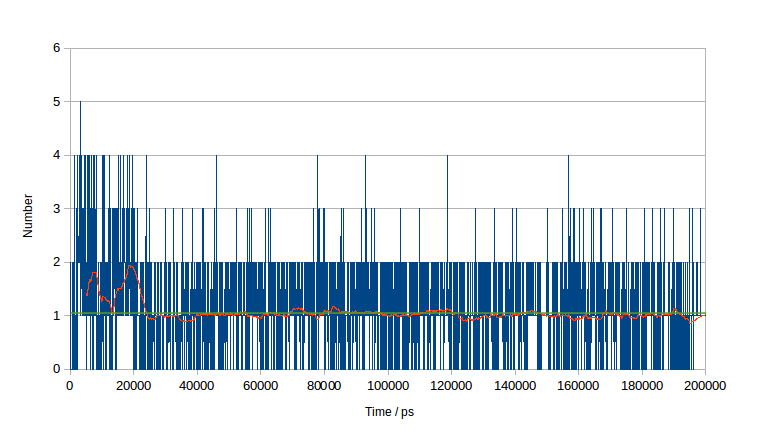
\includegraphics[width=0.9\textwidth, keepaspectratio=true]{graphics/HbondACP2_protein.png}}
		\caption[Number of hydrogen bonds formed between the ACP-mupA2 cognate substrate and the ACP-mupA2a surface residues over time.]{Number of hydrogen bonds formed between the ACP-mupA2 cognate substrate and the ACP-mupA2a surface residues.  Red line represents the running average over 500 frames and green line represents the mean.}
		\label{fig:HbondACP2_protein}
		\end{figure}

		\setlength\fboxsep{5pt}
		\setlength\fboxrule{1.5pt}
		\begin{figure}[htbp]
		\centering
		\fbox{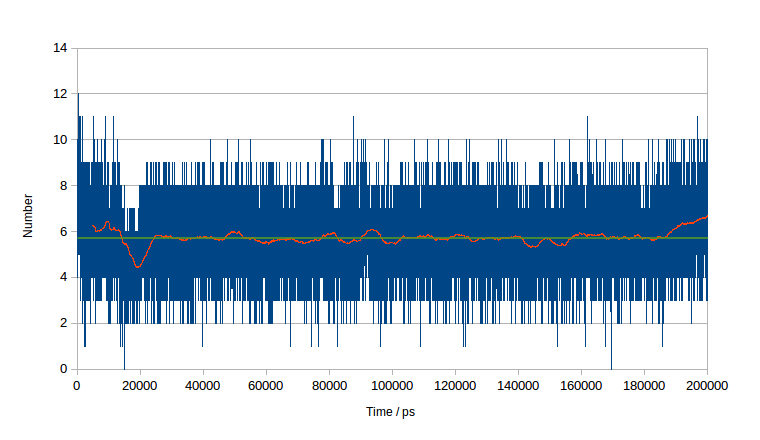
\includegraphics[width=0.9\textwidth, keepaspectratio=true]{graphics/HbondACP2_solvent.png}}
		\caption[Number of hydrogen bonds formed between the ACP-mupA2 cognate substrate and the solvent in the acyl ACP-mupA2a simulation.]{Number of hydrogen bonds formed between the ACP-mupA2 cognate substrate and the solvent in the acyl ACP-mupA2a simulation.  Red line represents the running average over 500 frames and green line represents the mean.}
		\label{fig:HbondACP2_solvent}
		\end{figure}

\newpage
	\subsection{Change in solvent accessible surface area of the ligand over time}
	\label{sec:AppIII:SASA}							

		\setlength\fboxsep{5pt}
		\setlength\fboxrule{1.5pt}
		\begin{figure}[htbp]
		\centering
		\fbox{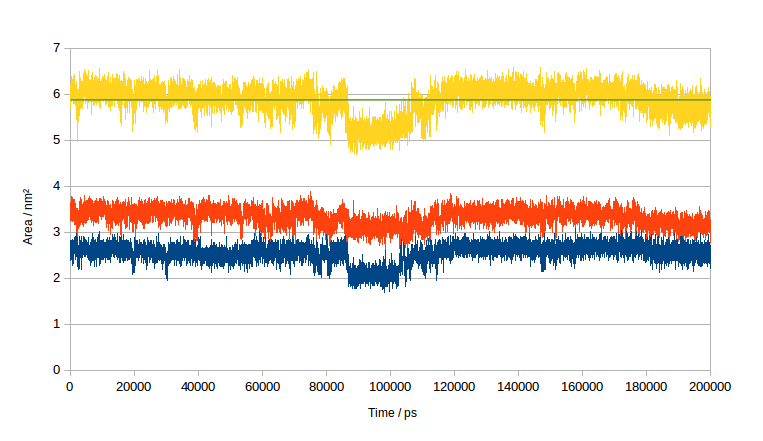
\includegraphics[width=0.9\textwidth, keepaspectratio=true]{graphics/sasACPPPTWild_area.png}}
		\caption[Change in the solvent accessible surface (SAS) of phosphopantetheine over time in the holo ACP-mupA3a WT simulation.]{Change in the solvent accessible area of phosphopantetheine over time in the holo ACP-mupA3a WT simulation. Blue line represents hydrophobic SAS, red line represents hydrophilic SAS, yellow line represents total SAS and green line represents the mean of the total SAS.}
		\label{fig:sasACPPPTWild_area}
		\end{figure}

		\setlength\fboxsep{5pt}
		\setlength\fboxrule{1.5pt}
		\begin{figure}[htbp]
		\centering
		\fbox{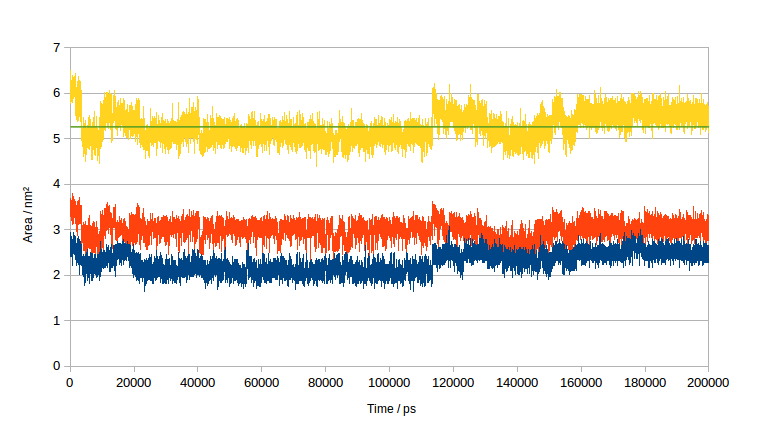
\includegraphics[width=0.9\textwidth, keepaspectratio=true]{graphics/sasACPPPTMutant_area.png}}
		\caption[Change in the solvent accessible surface (SAS) of phosphopantetheine over time in the holo ACP-mupA3a W44L simulation.]{Change in the solvent accessible surface (SAS) of phosphopantetheine over time in the holo ACP-mupA3a W44L simulation. Blue line represents hydrophobic SAS, red line represents hydrophilic SAS, yellow line represents total SAS and green line represents the mean of the total SAS.}
		\label{fig:sasACPPPTMutant_area}
		\end{figure}

		\setlength\fboxsep{5pt}
		\setlength\fboxrule{1.5pt}
		\begin{figure}[htbp]
		\centering
		\fbox{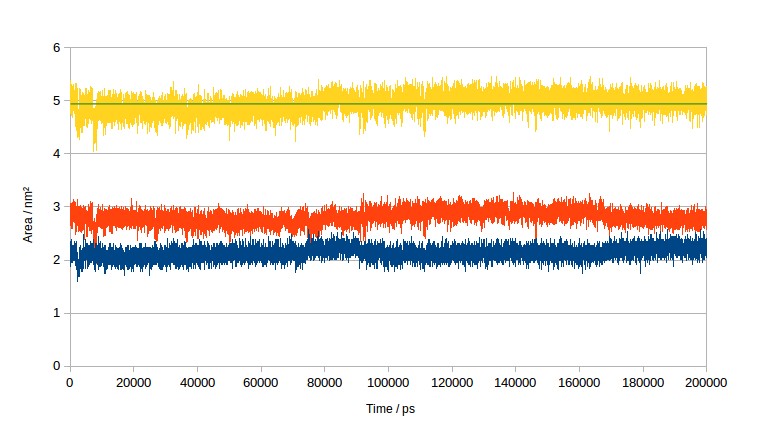
\includegraphics[width=0.9\textwidth, keepaspectratio=true]{graphics/sasACPSPMWild200_area.png}}
		\caption[Change in the solvent accessible surface (SAS) of the ACP-mupA3a cognate substrate over time (200 ns) in the acyl ACP-mupA3a WT simulation.]{Change in the solvent accessible area of the ACP-mupA3a cognate substrate over time (200 ns) in the acyl ACP-mupA3a WT simulation. Blue line represents hydrophobic SAS, red line represents hydrophilic SAS, yellow line represents total SAS and green line represents the mean of the total SAS.}
		\label{fig:sasACPSPMWild200_area}
		\end{figure}

		\setlength\fboxsep{5pt}
		\setlength\fboxrule{1.5pt}
		\begin{figure}[htbp]
		\centering
		\fbox{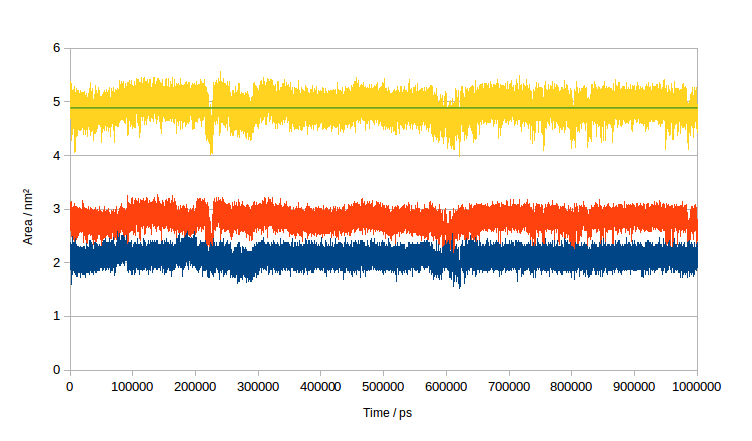
\includegraphics[width=0.9\textwidth, keepaspectratio=true]{graphics/sasACPSPMWild1000_area.png}}
		\caption[Change in the solvent accessible surface (SAS) of the ACP-mupA3a cognate substrate over time (1 $ \mu $s) in the acyl ACP-mupA3a WT simulation.]{Change in the solvent accessible surface (SAS) of the ACP-mupA3a cognate substrate over time (1 $ \mu $s) in the acyl ACP-mupA3a WT simulation.. Blue line represents hydrophobic SAS, red line represents hydrophilic SAS, yellow line represents total SAS and green line represents the mean of the total SAS.}
		\label{fig:sasACPSPMWild1000_area}
		\end{figure}
		
		\setlength\fboxsep{5pt}
		\setlength\fboxrule{1.5pt}
		\begin{figure}[htbp]
		\centering
		\fbox{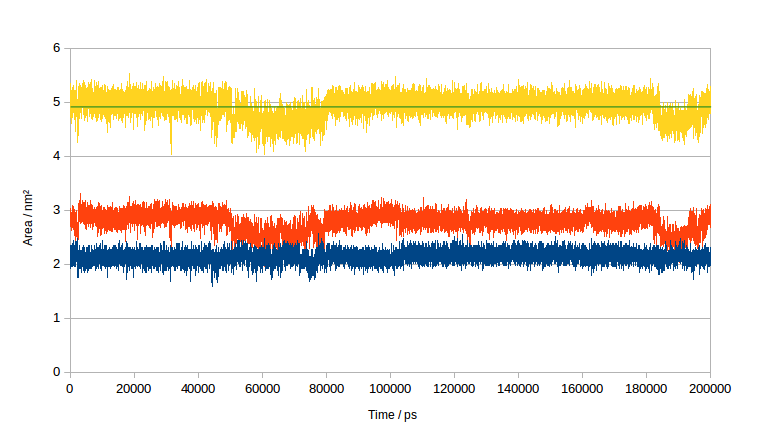
\includegraphics[width=0.9\textwidth, keepaspectratio=true]{graphics/sasACPSPMMutant_area.png}}
		\caption[Change in the solvent accessible surface (SAS) of the ACP-mupA3a cognate substrate over time in the acyl ACP-mupA3a W44L simulation.]{Change in the solvent accessible surface (SAS) of the ACP-mupA3a cognate substrate over time in the acyl ACP-mupA3a W44L simulation. Blue line represents hydrophobic SAS, red line represents hydrophilic SAS, yellow line represents total SAS and green line represents the mean of the total SAS.}
		\label{fig:sasACPSPMMutant_area}
		\end{figure}

		\setlength\fboxsep{5pt}
		\setlength\fboxrule{1.5pt}
		\begin{figure}[htbp]
		\centering
		\fbox{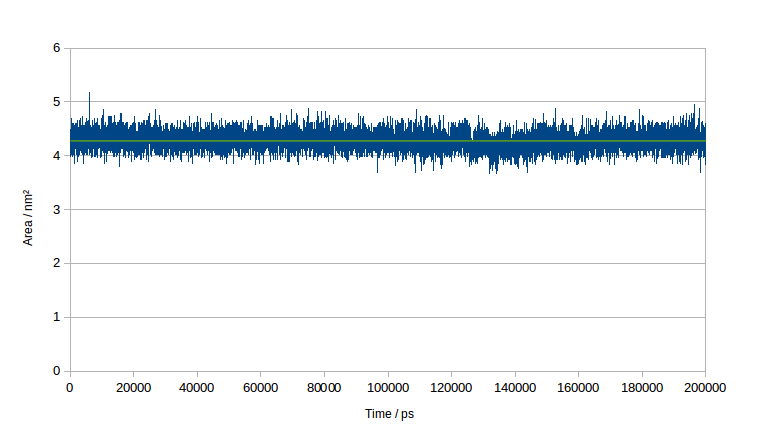
\includegraphics[width=0.9\textwidth, keepaspectratio=true]{graphics/sasACPSPD_area.png}}
		\caption[Change in the solvent accessible surface (SAS) of the 14C saturated chain over time in the acyl 14C ACP-mupA3a simulation.]{Change in the solvent accessible surface (SAS) of the 14C saturated chain over time in the acyl 14C ACP-mupA3a simulation. Blue line represents hydrophobic SAS and green line represents the mean of the total SAS.}
		\label{fig:sasACPSPD_area}
		\end{figure}

		\setlength\fboxsep{5pt}
		\setlength\fboxrule{1.5pt}
		\begin{figure}[htbp]
		\centering
		\fbox{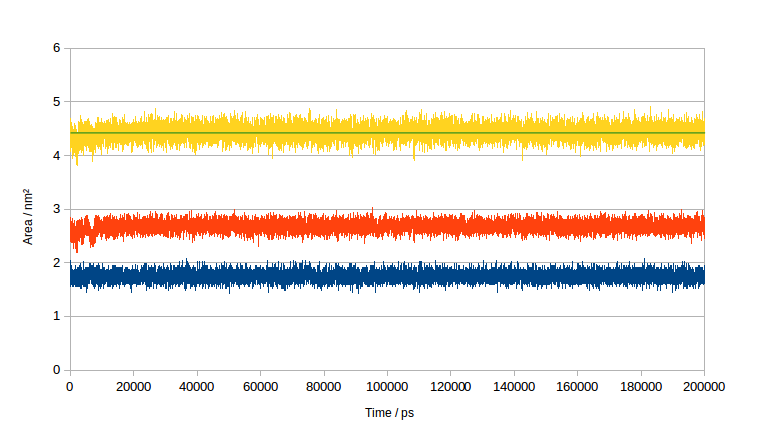
\includegraphics[width=0.9\textwidth, keepaspectratio=true]{graphics/sasACP2_area.png}}
		\caption[Change in the solvent accessible surface (SAS) of the ACP-mupA2 cognate substrate over time in the acyl ACP-mupA2a simulation.]{Change in the solvent accessible surface (SAS) of the ACP-mupA2 cognate substrate over time in the acyl ACP-mupA2a simulation. Blue line represents hydrophobic SAS, red line represents hydrophilic SAS, yellow line represents total SAS and green line represents the mean of the total SAS.}
		\label{fig:sasACP2_area}
		\end{figure}		

\clearpage
	\subsection{Sequence logos}
	\label{sec:sequence logos}		
	On the next page. 
		
		\setlength\fboxsep{5pt}
		\setlength\fboxrule{1.5pt}
		\begin{sidewaysfigure}[htbp]
		\centering
		\fbox{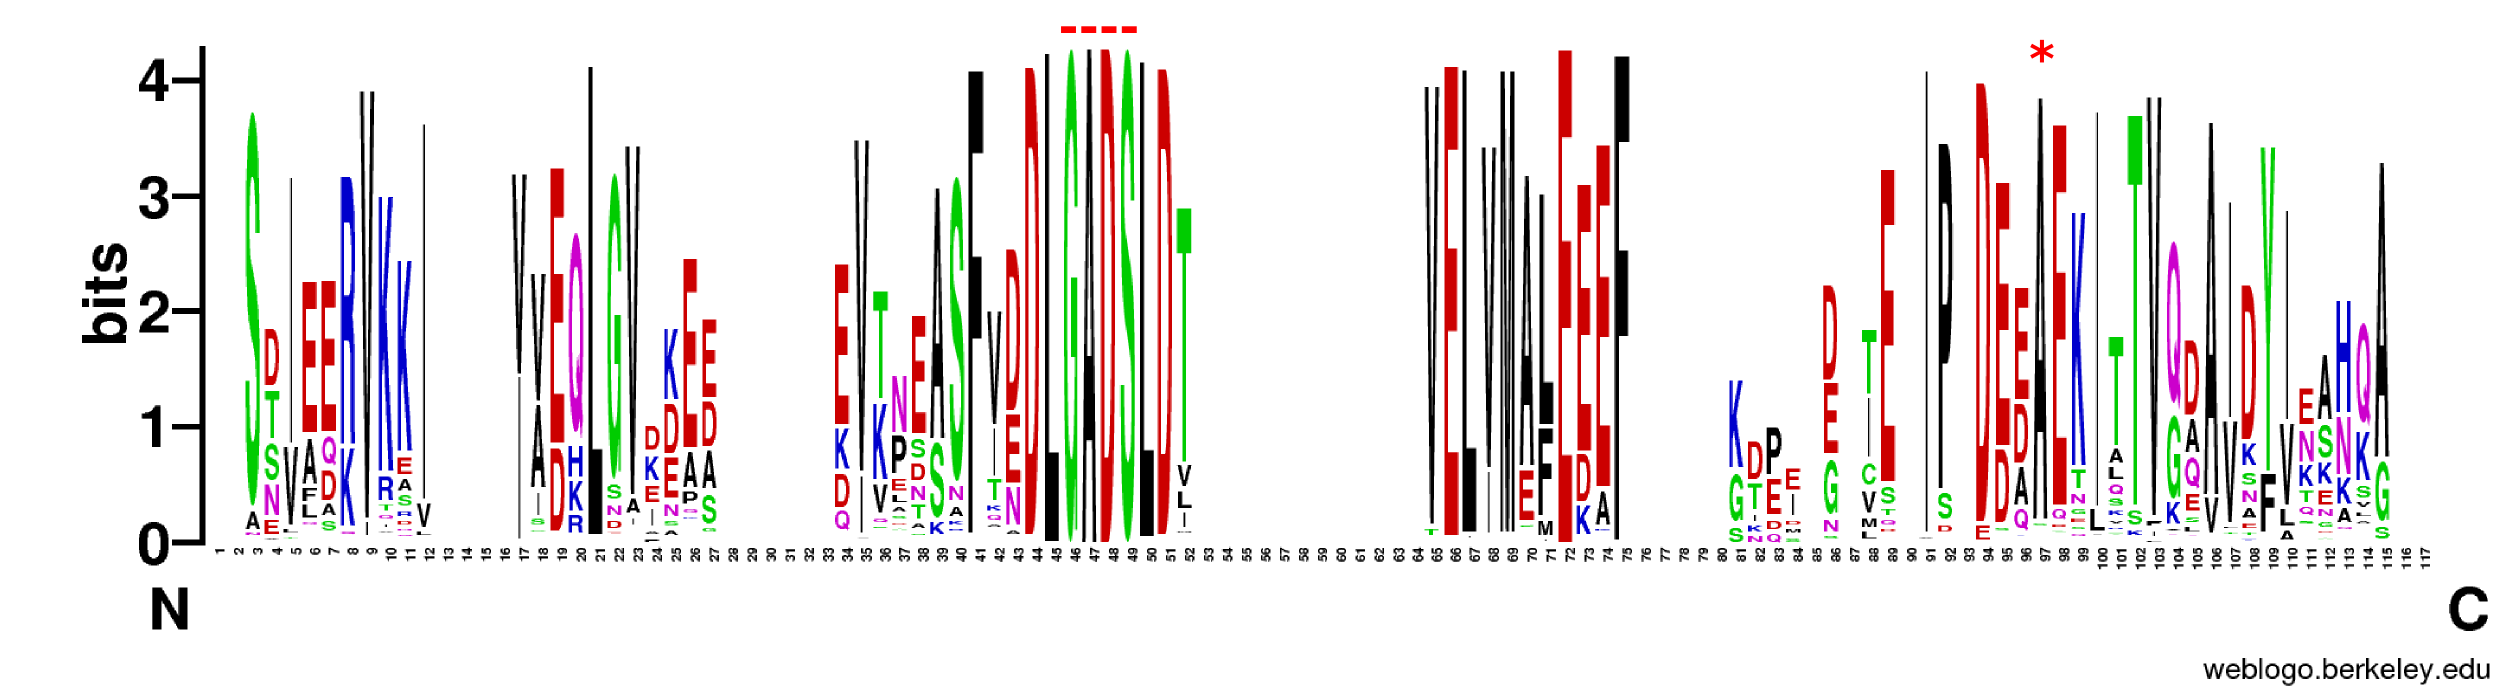
\includegraphics[width=\textwidth, keepaspectratio=true]{graphics/gadsnopattern.png}}
		\caption[Sequence logo built on 2078 unique FAS ACP sequences with GADS motif.]{Sequence logo built on 2078 unique FAS ACP sequences with GADS motif. These sequences were searched with normal BLASTp without any pattern and post search filtered for sequences carrying GADS motif. \textcolor{red}{- - - - -} indicates the GADS position and \textcolor{red}{*} indicates the position equivalent to A59 in the FAS ACPs.}
		\label{fig:gadsnopattern}
		\end{sidewaysfigure}	

		\setlength\fboxsep{5pt}
		\setlength\fboxrule{1.5pt}
		\begin{sidewaysfigure}[htbp]
		\centering
		\fbox{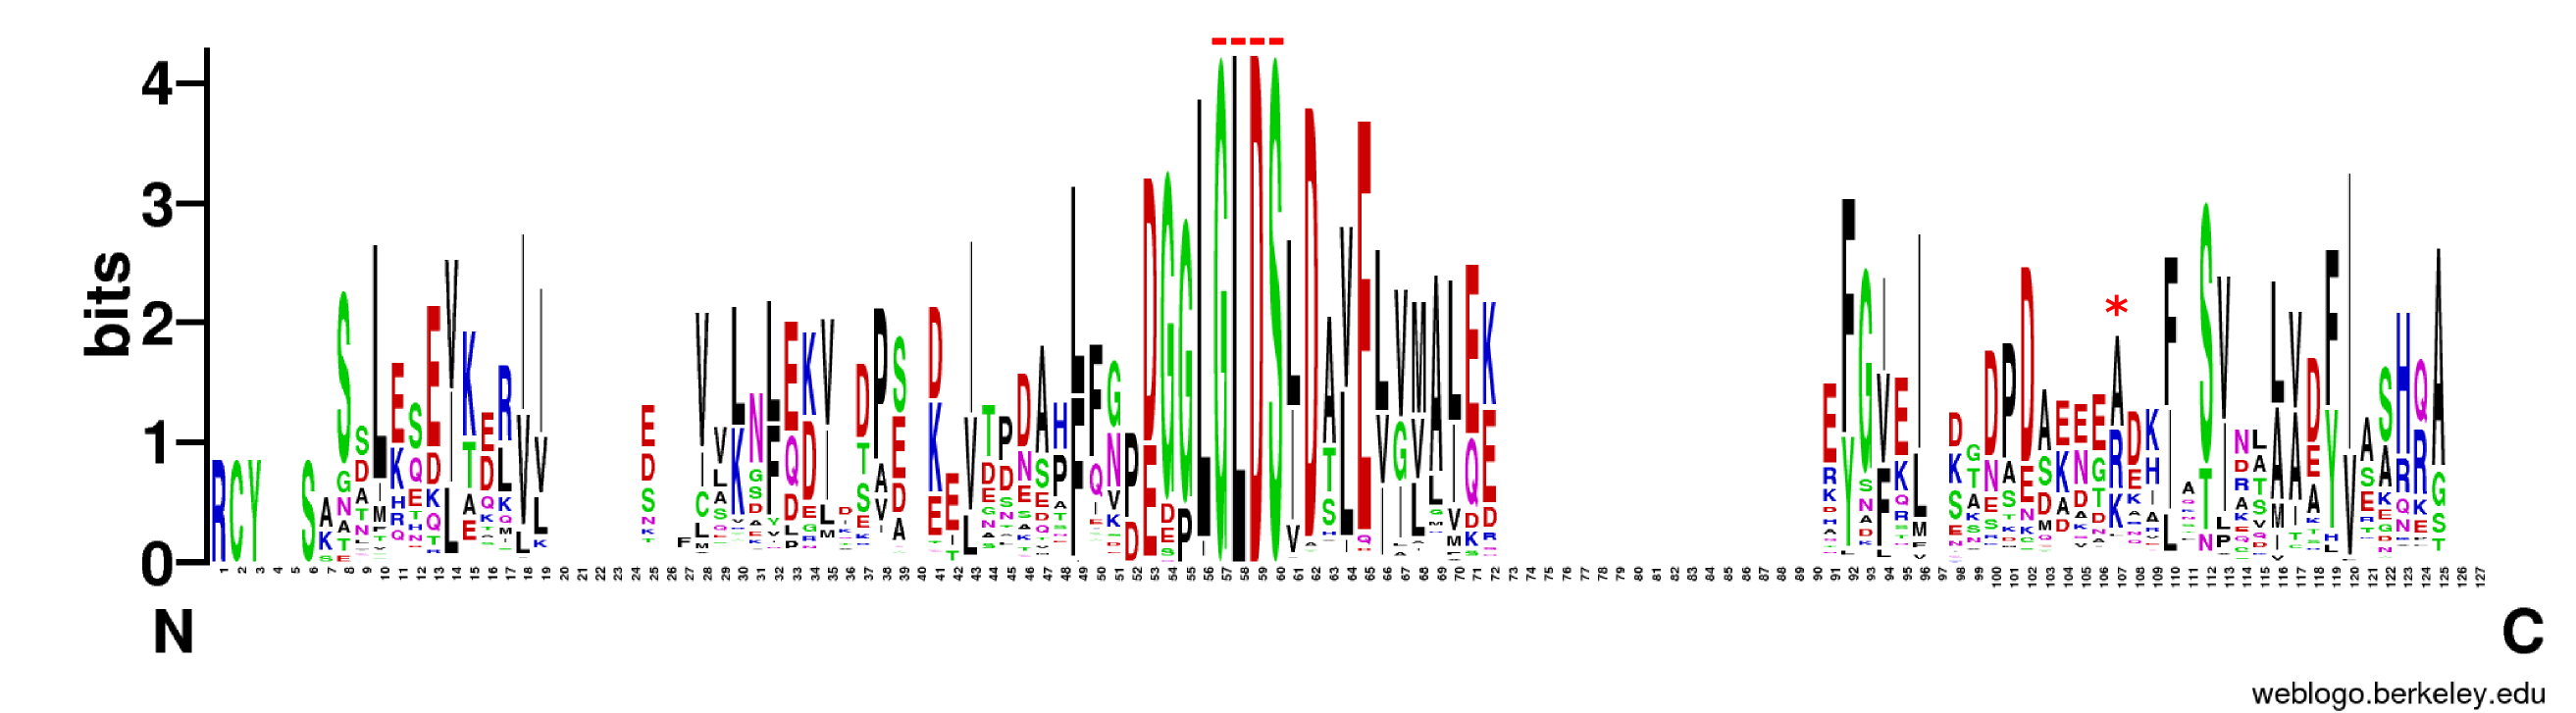
\includegraphics[width=\textwidth, keepaspectratio=true]{graphics/gldsnopattern.png}}
		\caption[Sequence logo built on 257 unique FAS ACP sequences with GLDS motif.]{Sequence logo built on 257 unique FAS ACP sequences with GLDS motif. These sequences were searched with normal BLASTp without any pattern and post search filtered for sequences carrying GLDS motif. \textcolor{red}{- - - - -} indicates the GLDS position and \textcolor{red}{*} indicates the position equivalent to A59 in the FAS ACPs.}
		\label{fig:gldsnopattern}
		\end{sidewaysfigure}			

		\setlength\fboxsep{5pt}
		\setlength\fboxrule{1.5pt}
		\begin{sidewaysfigure}[htbp]
		\centering
		\fbox{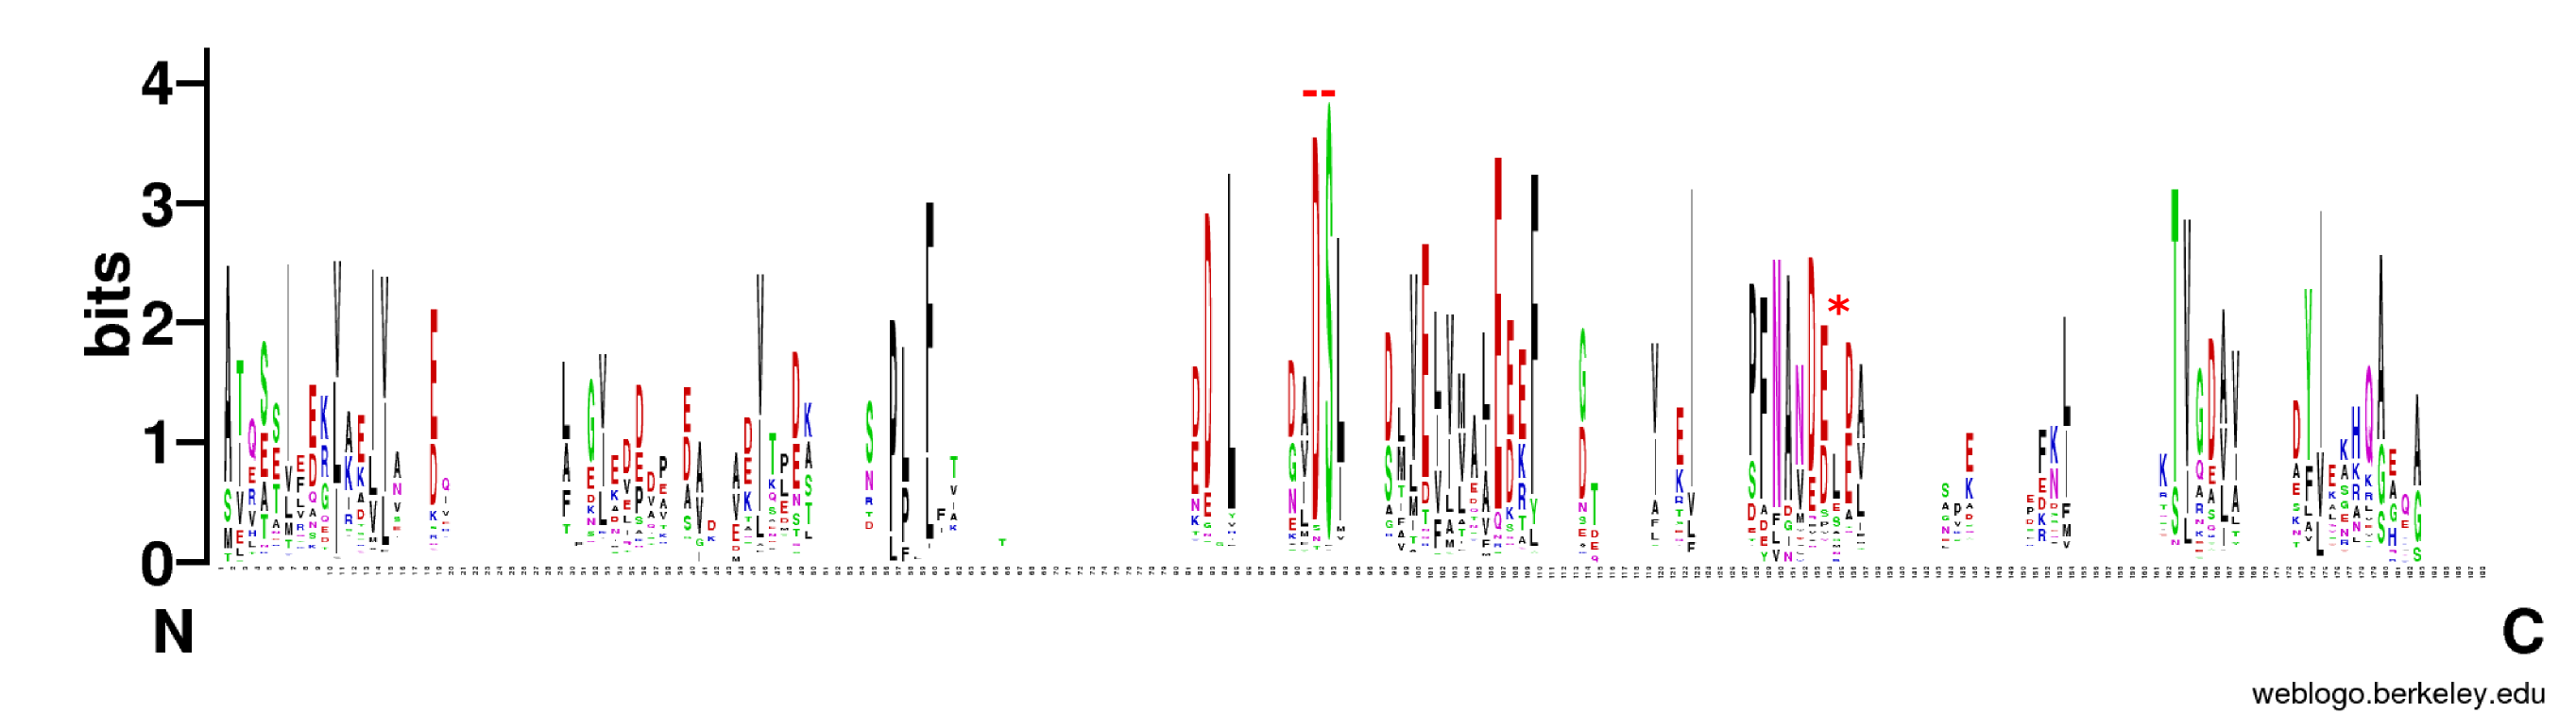
\includegraphics[width=\textwidth, keepaspectratio=true]{graphics/neithernopattern.png}}
		\caption[Sequence logo built on 541 unique FAS ACP sequences with neither GADS or GLDS motif.]{Sequence logo built on 541 unique FAS ACP sequences with neither GADS or GLDS motif. These sequences were searched with normal BLASTp without any pattern and post search filtered for sequences devoid of GADS or GLDS motif. \textcolor{red}{- - - - -} indicates the GXDS position and \textcolor{red}{*} indicates the position equivalent to A59 in the FAS ACPs.}
		\label{fig:neithersnopattern}
		\end{sidewaysfigure}			


							
									
\end{singlespacing}